% This file is for chapter 3

\chapter{Automatic Parallel Portfolio Selection}

A portion of this chapter has been published as: H. Kashgarani, L. Kotthoff, “Automatic Parallel Portfolio Selection,” in \textit{ECAI 2023}, pp. 1215-1222, IOS Press, 2023.

This chapter introduces a hybrid formulation for dynamic algorithm portfolio selection, which is instance-based and aims to mitigate the risk of selecting a single algorithm or running too many solvers in parallel. The published ECAI paper investigates the results for a random forest regression model trained using the MLR package. Here, in addition to presenting those results, we also expand upon them to explore the transition of regression random forests from the MLR package to its updated version, MLR3, in R.

\section{Abstract}
Algorithms to solve hard combinatorial problems often exhibit complementary performance, i.e.\ where one algorithm fails, another shines. Algorithm portfolios and algorithm selection take advantage of this by running all algorithms in parallel or choosing the best one to run on a problem instance. In this chapter, we show that neither of these approaches gives the best possible performance and propose the happy medium of running a subset of all algorithms in parallel. We propose a method to choose this subset automatically for each problem instance, and demonstrate empirical improvements of up to 23\% in terms of runtime, 83\% in terms of misclassification penalty, and 32\% in terms of penalized averaged runtime on scenarios from the ASlib benchmark library. Unlike all other algorithm selection and scheduling approaches in the literature, our performance measures are based on the actual performance for algorithms running in parallel rather than assuming overhead-free parallelization based on sequential performance. Our approach is easy to apply in practice and does not require to solve hard problems to obtain a schedule, unlike other techniques in the literature, while still delivering superior performance.

\section{Introduction}
For many types of hard combinatorial problems, different algorithms that exhibit complementary performance are available. In these cases, a portfolio of algorithms often achieves better performance than a single one \cite{Huberman1997,GOMES200143}. The algorithms can be run in parallel, or a single one selected for each problem instance to solve. The so-called Algorithm Selection Problem \cite{Rice1976} is often solved using machine learning models which, given characteristics of the problem instance to solve, decide which algorithm should be chosen \cite{Kotthoff2014,10.1162/evco_a_00242}. The machine learning models built for per-instance algorithm selection are not perfect, like most models. In some cases, they lead to choosing an algorithm that does not provide the best overall performance, resulting in wasted resources.

Running all algorithms in parallel avoids this issue, but again wastes resources. Even if the user is only interested in optimizing the elapsed time, i.e.\ it does not matter how many things are run in parallel, results are sub-optimal as parallel executions compete for shared resources such as caches. With more solvers running in parallel, more runs time out, which results in a large overhead. Even for a relatively small number of parallel runs, this overhead becomes prohibitive, resulting in overall performance worse than using imperfect machine learning models to choose a single algorithm \cite{pmlr-v140-kashgarani21a}.

In this chapter, we propose a middle path -- select the most promising subset of algorithms to be run in parallel on a single non-distributed computing machine. This mitigates the impact of both imperfect machine learning models and overhead from parallel runs. We formalize the problem of choosing a subset of algorithms from a portfolio, unifying approaches from the literature. We propose a solution to this problem based on the predictions of algorithm performance models and their uncertainties and compare empirically to other approaches from the literature. We trained three algorithm selection performance models and applied the proposed formulation and could demonstrate improvements of up to 83\% in terms of misclassification penalty, establishing a new state of the art in per-instance algorithm selection with multiple algorithms. We assume that the algorithms to run are not parallelized themselves, i.e.\ each algorithm consumes the same computational resources, and we run on a single machine. We do not consider the case of running algorithms in a distributed setting on multiple machines.

\subsection{Algorithm Selection}
The performance of algorithms designed to solve NP-complete problems, such as Boolean Satisfiability and the Traveling Salesman Problem, can vary significantly depending on the specific problem being addressed. There is no one algorithm that performs optimally in all circumstances. However, we can take advantage of these performance disparities by creating algorithm portfolios that incorporate the complementing strengths of several algorithms \cite{GOMES200143,Huberman1997}. 

The algorithm portfolios proposed in \cite{GOMES200143,Huberman1997} run multiple algorithms in parallel, however, they do not measure the actual execution time when running in parallel but simulate parallel execution based on sequential performance. \cite{pmlr-v140-kashgarani21a} found that the performance of the portfolio can deteriorate substantially when algorithms are executed in parallel, in particular for more than 10 algorithms. \cite{LINDAUER2017272} has also determined that running various configurations of an algorithm in parallel can introduce overhead, and this factor should be considered when designing portfolios. Alternatively, we can choose a subset of the best algorithms from the portfolio for a given problem instance to avoid the overhead of running a large number of solvers in parallel. In the case where we choose only a single algorithm, this is known as the algorithm selection problem~\cite{Rice1976}. Typically, this is accomplished through the use of machine learning techniques and features derived from the instances~\cite{Kotthoff2014,10.1162/evco_a_00242} and algorithms~\cite{pmlr-v188-pulatov22a}. However, choosing only a single algorithm to run often achieves suboptimal performance because of incorrect choices. This can be addressed through better algorithm selection models; in this chapter, we explore the alternative of choosing more than one algorithm to run in parallel on a single node.

Algorithm selection has been applied successfully in many problem domains. Some of the most prominent systems are SATzilla, Hydra, and Autofolio ~\cite{satzilla,lindauer2015autofolio,10.5555/2898607.2898641}. While these systems focus on SAT, algorithm selection also has been used in the constraint programming and mixed integer programming domains, where it has been shown to achieve good performance \cite{cphydra,XuEtAl11}. AutoFolio has been applied in additional areas, e.g.\ ASP, MAXSAT, and QBF. \cite{10.1162/evco_a_00215} apply algorithm selection for the TSP, and ME-ASP \cite{maratea2014multi} apply algorithm selection for answer set programming to create a multi-engine solver. Algorithm selection has also been used to choose between evolutionary algorithms \cite{HU201268, yuen2019selecting, Maturana2012, 9ae8443ad82b4056bccf7102c0056152}.
The ASlib benchmarking library~\cite{BISCHL201641} collects benchmarks from many different problem domains and is the de facto standard library for evaluating algorithm selection approaches.

\par{\textbf{Notation.}}
We follow~\cite{pmlr-v79-lindauer17a} in the notation we use in this chapter.
Given a portfolio of algorithms (solvers) $S$, a set of instances $I$, and a performance metric \begin{math} m: S \times I \to \mathbb {R^+} \end{math}, we aim to find a mapping \begin{math} s: I \to S \end{math} from instances $I$ to algorithms $S$ such that the performance across all instances is optimized. This performance metric can be for example the time needed to solve the instance and we assume w.l.o.g.\ that the performance metric should be minimized. In practice, we estimate the value of the performance metric based on the predictions of machine learning models for new problem instances; we denote this estimate $\hat{m}$. We want to select the solver with the best-predicted performance for each instance:

\begin{equation}\label{eq:1}
    min \frac{1}{|I|} \sum\limits_{i\in I} \hat{m}(s(i),i)
\end{equation}


\subsection{Portfolio Scheduling}
Different approaches have been proposed for sub-portfolio selection. Some approaches choose a number of suitable solvers for sequential execution and assign  time slices that sum to the total available time to each algorithm. Others have implemented parallel execution of the selected solvers, while a few have combined these two methods, utilizing parallelization across computing processors and splitting the available time of each processor across different algorithms. 

\subsubsection{Time slice allocation on single processor}

Typically, sub-portfolio selection strategies are built for sequential solver runs, e.g.\ Sunny~\cite{sunny} creates a sub-portfolio of solvers using k-nearest neighbor (kNN) models and builds a sequential schedule for the selected solvers by allocating time slices based on the predicted performance. CPHydra~\cite{cphydra} also employs case-based reasoning and allocates time slices for the selected CSP solvers to run sequentially. 3S~\cite{3s} dynamically selects and sequentially schedules solvers for a given SAT instance using integer programming. ASPEED~\cite{aspeed} creates static sequential schedules through answer set programming that optimizes a static sequential time budget allocation for solvers. Depending on the number of algorithms, solving the scheduling problem can take substantial time. Building on the methodologies of 3S~\cite{3s} and ASPEED~\cite{aspeed}, ISA (Instance-Specific ASPEED)~\cite{flexfolio} uses kNN to identify the closest training problem instances to a given problem instance to solve. It then employs ASPEED to determine a schedule that minimizes the number of timeouts across these instances. \cite{flexfolio} also introduced TSunny which is a modified version of Sunny that limits the number of solvers to run, thus increasing the chance of success by allocating larger time slices to each algorithm.

\subsubsection{Time slice allocation on multiple processors}

Other portfolio techniques have focused on scheduling solvers to run in parallel and allocating time slots on different processors. P3S~\cite{p3s} is a parallel version of 3S and uses the kNN algorithm for selecting solvers and scheduling them using integer programming with a specific runtime allocation strategy, where it runs a static set of solvers for the first 10\% of the available runtime and solvers selected for the instance for the remaining 90\%. ASPEED~\cite{aspeed} can also define a fixed schedule for running solvers on multiple processors, which is chosen based on the average solver performance across a set of instances. Flexfolio \cite{flexfolio} incorporates a reimplementation of the P3S approach utilizing the same 10-90 strategy. However, rather than employing integer programming to address the scheduling problem, Flexfolio makes use of ASPEED and solves it through answer set programming. Sunny-cp~\cite{sunnycp2} can simultaneously execute multiple CSP and COP solvers. First, a portion of the total available time is allocated to a pre-solving phase that follows a fixed schedule. The remaining time is then distributed amongst the other selected solvers dynamically, based on the predictions of kNN performance models. As there are often more solvers than processors, all processors except one are assigned to the corresponding number of top-ranked solvers, while the time on the final processors is split among the remaining solvers.

\subsubsection{Running algorithms in parallel}

One of the first parallel SAT solvers is ppfolio~\cite{ppfolio}. It selects solver portfolios to solve sets of problem instances optimally, but does this only for entire sets of instances, not on a per-instance basis as we do here.
The success of ppfolio has inspired many other researchers to create sub-portfolios of solvers to run in parallel. For example, \cite{Marius2015} extended existing algorithm selectors like 3S, SATzilla, and ME-ASP to greedily choose the top $n$ solvers to run in parallel by producing a ranking of candidate algorithms; however, the number of solvers has to be specified by the user and the actual runtime of parallel runs is not considered -- the same runtime as for sequential execution is assumed.
Running algorithms in parallel on the same machine is slower than running sequentially in practice due to the overhead incurred because of shared caches and shared memory. This has been shown in experiments~\cite{pmlr-v140-kashgarani21a}, simulations~\cite{Yun,jtom1286288}, and analyses~\cite{biere} for the parallel executions of solvers -- in practice, ignoring the overhead that parallel execution introduces reduces overall performance.

\medskip

In this chapter, we consider the problem of selecting the optimal subset of algorithms to run in parallel on a single machine. This is computationally much easier to solve on a per-instance basis than more complex scheduling approaches, e.g.\ the ones used by ASPEED and 3S, which means that our method is easier to deploy and introduces less overhead. As long as the best solver is part of the selected portfolio, we will achieve optimal performance or close to it, whereas approaches that allocate time slices may choose the best solver, but fail to achieve optimal performance if too little time is allocated to it. We leverage more information from algorithm selection models than most approaches in the literature, in particular the uncertainty of performance prediction. This allows us to trade off the number of algorithms to choose with the chance of success in a principled way. Our approach is designed to optimize the usage of parallel computational resources when solving combinatorial problems while taking into account the overhead that arises from parallel runs. To the best of our knowledge, there are no other approaches that solve parallel algorithm selection this way.

\section{Parallel Portfolio Selection}

We aim to choose a sub-portfolio of solvers \begin{math} P_i \subseteq S \end{math} for a given instance $i \in I$ that includes the algorithms with the best performance on $i$ (\begin{math} A \in S \end{math} and \begin{math} A \in P_i \end{math}) to run in parallel, based on the predicted performance of each solver. Given the predicted performance metric $\hat{m}$, we can define a total order of the algorithms in the portfolio $S$ for a given instance $i$. This total order is induced by the ranking of the algorithms based on their predicted performance for instance $i$. Formally, the total order can be defined as:
\begin{equation}\label{eq:3}
A < B \quad \text{if} \quad \hat{m}(A,i) < \hat{m}(B,i); A,B \in S
\end{equation}

Given the total order, the rank of each algorithm $A$ on each instance $i$ can be defined as the number of algorithms that are predicted to be strictly better than $A$ for the instance and denoted $r_{A,i}$. Ties are broken arbitrarily. A portfolio of a specified size $n$ is then defined as the top $n$ algorithms according to rank for that particular instance. The portfolio of size $n$ for instance $i$ can be expressed mathematically as:
\begin{equation}\label{eq:4}
P_i = \{A \in S \: | \: r_{A,i} \leq n\}
\end{equation}

In a slight abuse of notation, we will denote the rank of an algorithm as a subscript, i.e.\ $r_{A,i}$ is the rank of algorithm $A$ on instance $i$ and $A_{1,i}$ is the algorithm of rank $1$ (the best performing algorithm) on instance $i$.

This allows to choose a subset of algorithms with the best predicted performance for a given instance, which can then be executed in parallel. However, determining the portfolio size $n$ for a given problem instance is the key challenge for parallel portfolios. As discussed above, choosing only a single algorithm or all algorithms is unlikely to give optimal performance in practice. The larger the number of algorithms we include, the larger the chance that the best algorithm is in the chosen portfolio, but also the larger the overhead from running many algorithms in parallel. 

Here, we want to include the algorithms that, according to their predicted performance on a new problem instance, have the highest chances of achieving optimal performance, while also taking into account the computational overhead of running multiple solvers in parallel. We leverage the uncertainty of the predictions of the performance models to gauge the likelihood that a given algorithm would be competitive. To the best of our knowledge, there are no algorithm selection approaches that do this.

Instead of considering only a point prediction, we consider the predicted distribution of performance metric values, characterized by its mean and standard deviation. Formally, we denote the standard deviation of the prediction \begin{math}\hat{m}(A, i)\end{math} as \begin{math}\sigma_{A, i}\end{math} for each solver $A$ and instance $i$.
We assume that the predictions of our performance models follow a normal distribution, i.e.\ the predicted value is the mean of that distribution and allows to characterize it completely together with the standard deviation. We assess the likelihood of two algorithms performing equally well by computing the overlap between their distributions. If two algorithms are predicted to perform very similarly, then the overlap between the distributions will be very large.

We are in particular interested in the predicted performance distribution of the best-predicted algorithm $A_{1,i}$ (no algorithms are predicted to perform better than it), and how the predictions for the other algorithms compare to it.
Formally, for the best predicted solver $A_{1,i}$ on instance $i$ the distribution of predictions is \begin{math} \hat{m}(A_{1,i}, i) \sim \hat{M}(\mu_{A_{1,i},i}, \sigma^2_{A_{1,i},i}) \end{math} with probability density function \begin{math} f_{A_{1,i},i}\end{math} and cumulative distribution function \begin{math} F_{A_{1,i},i}\end{math}. The performance distributions for other algorithms are defined similarly.

For the distributions of the predicted performance of two algorithms $A_x$ and $A_y$ on instance $i$, the point of intersection $c$ can be computed as \begin{math} f_{A_x,i}(c) =  f_{A_y,i}(c) \end{math}. That is, the predicted probability of achieving this particular performance is equal for both distributions (illustrated in Figure~\ref{fig:overlappingarea}).
For \begin{math}
    \mu_{A_x,i} < \mu_{A_y,i}
\end{math}, $c$ is defined as (we omit the index $i$ for the sake of brevity here):

\begin{equation}\label{eq:5}
\resizebox{\columnwidth}{!}{$c = \frac{\mu _{A_y} \sigma _{A_x}^2-\sigma _{A_y} \left(\mu _{A_x} \sigma _{A_y}+\sigma _{A_x} \sqrt{\left(\mu _{A_x}-\mu _{A_y}\right){}^2+2 \left(\sigma _{A_x}^2-\sigma _{A_y}^2\right) \log \left(\frac{\sigma _{A_x}}{\sigma _{A_y}}\right)}\right)}{\sigma _{A_x}^2-\sigma _{A_y}^2}$}
\end{equation}

Given $c$, the overlap between the distributions is defined as the joint probability of $A_x$ performing worse than $c$ and $A_y$ performing better than $c$:

\begin{equation}\label{eq:6}
    p(\hat{m}({A_{x,i}}, i) \geq c) \cdot p(\hat{m}({A_{y,i}}, i) \leq c) = 1 - F_{A_{x,i},i}(c) +  F_{A_{y,i},i}(c)
\end{equation}

We define $p_{\cap} \in [0,1]$ as a threshold for the computed joint probability to include a given algorithm:

\begin{equation}\label{eq:7}
 P_i = \{A \:| \: \left(p(\hat{m}({A_{1,i},i)} \geq c) \: \cdot \: p(\hat{m}({A_{x,i}}, i) \leq c)\right) \geq \:p_{\cap}\:\}
\end{equation}

$p_{\cap}$ is 1 for the best predicted algorithm, and 0 for algorithms whose distribution does not have any overlap with that of the best predicted algorithm, i.e.\ the probability of performing at least as good as the best predicted algorithm is 0.

We can control the size of the parallel portfolio by adjusting the value of $p_{\cap}$. If $p_{\cap}$ is set to 1, only the best predicted algorithm and ones that are predicted to perform exactly like it are included. On the other hand, if $p_{\cap}$ is set to 0, all algorithms will be included. This allows us to tune our approach to a given algorithm selection scenario and choose the algorithms to run in parallel very flexibly, also accommodating potentially inaccurate performance predictions.

\begin{figure}
\centering
    \centerline{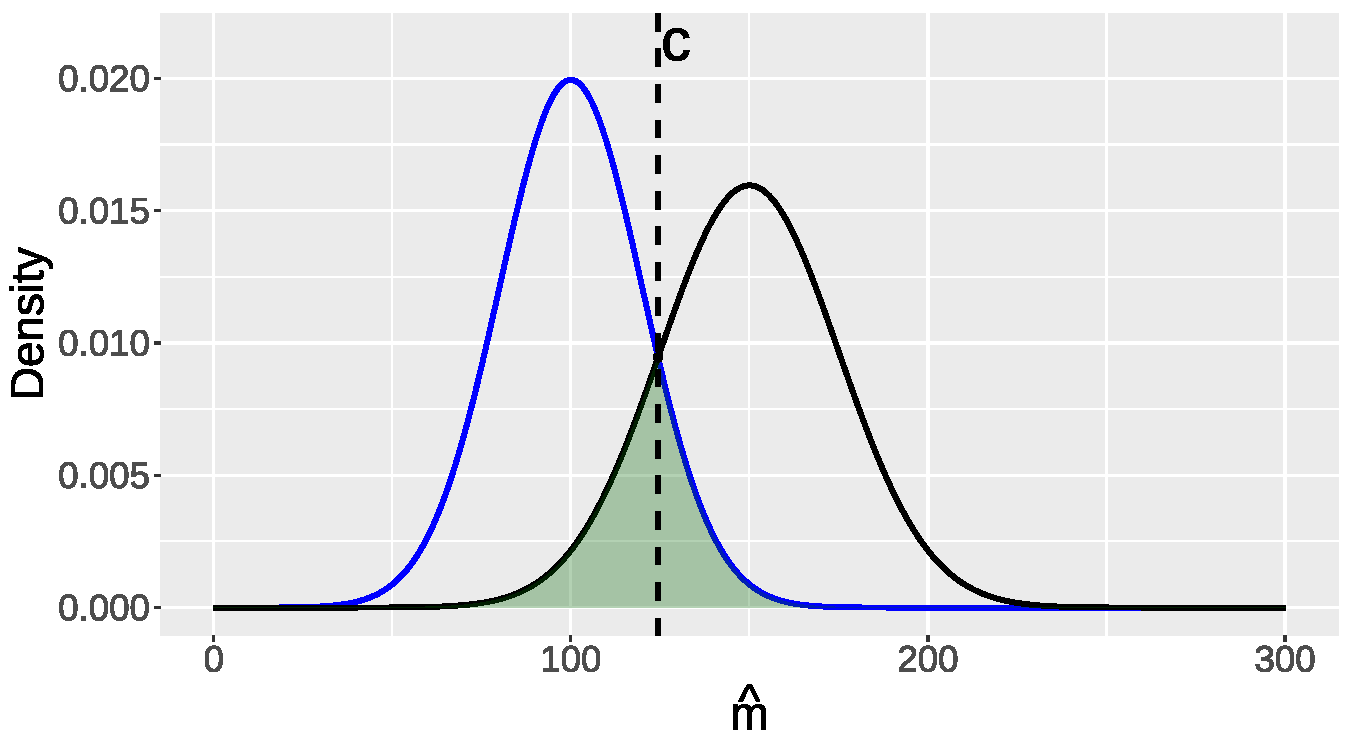
\includegraphics[width=0.8\linewidth]{plots/ovelappingarea.pdf}}
    \caption[Overlapping area of two normal distributions]{Overlapping area of two normal distributions. The point $c$ is the performance both distributions are equally likely to achieve. The shaded area denotes the probability of overlap between the two distributions; in our case, the probability that the candidate solver will perform as least as well as the best predicted solver.}
    \label{fig:overlappingarea}
\end{figure}

\section{Experimental Setup}
\subsection{Data Collection}

We used three scenarios from the ASlib benchmark repository ~\cite{BISCHL201641}: MAXSAT19-UCMS, SAT11-INDU, and SAT18-EXP. Additionally, we created two new scenarios: SAT16-MAIN, which utilizes solvers and instances from the SAT Competition 2016, and IPC2018, which incorporates solvers and instances from the International Planning Competition 2018. As ASlib only offers algorithm performance data for single runs, we conducted our own measurements for parallel runs on individual machines. We also measured the performance for single runs again and repeated the instance feature extraction steps to ensure that all experiments were performed on the same hardware. For MAXSAT19-UCMS, SAT11-INDU\footnote{For SAT11-INDU, the ASlib benchmark repository contains 115 extracted features, including those from SATZilla. However, we were unable to find the feature extraction for this scenario and used the same 54 instance features extracted by SATZilla.}, SAT16-MAIN, and SAT18-EXP, we used SATZilla’s feature computation code~\cite{satzilla}, and extracted 54 different features. For IPC2018 we used the feature extraction code by~\cite{Fawcett_Vallati_Hutter_Hoffmann_Hoos_Leyton-Brown_2014} which extracts 305 features for planning problems in PDDL format. We excluded 26 instances of SAT Competition 2016 from the SAT16-MAIN scenario because we were unable to extract features within two hours of computational time. 
We also omitted two solvers, glocusePLE and Scavel\_SAT, from SAT16-MAIN because of frequent out-of-memory errors on multiple instances. From IPC2018, we omitted three solvers, MSP, maplan-1, and maplan-2, because they require an unavailable version of CPLEX. Table~\ref{tab:scenarios} gives an overview of the scenarios, algorithms, instances, and features we use in our evaluation.

\begin{table}
\centering
\caption{Number of Algorithms, Instances, and Features Across All Scenarios.}
\label{tab:scenarios}
\begin{tabular}{p{5cm} cccc}
\toprule
Scenario & Algorithms & Instances & Instance Features\\
\midrule
IPC2018 & 15 & 240 & 305\\
MAXSAT19-UCMS & 7 & 572 & 54\\
SAT11-INDU & 14 & 300 & 54\\
SAT16-MAIN & 25 & 274 & 54\\
SAT18-EXP & 37 & 353 & 54\\
\bottomrule
\end{tabular}
\end{table}

We ran all solvers on all instances on compute nodes with 32 processors and 40 MB cache size (Intel(R) Xeon(R) CPU E5-2683 v4 @ 2.10GHz), 128 GB memory, and Red Hat Linux version 8.6. We use the same time limits as in the ASlib scenarios; 5000 CPU seconds for SAT18-EXP and SAT11-INDU, and 3600 CPU seconds for MAXSAT19-UCMS. For the new scenarios, we use the same time limits as the respective competitions; 5000 CPU seconds for SAT16-MAIN and 1800 CPU seconds for IPC2018. We ran each algorithm individually with 2-10 parallel runs. For all experiments, we ensured that only the given number of parallel runs were executed on a single machine. As our previous work showed that performance becomes worse than algorithm selection of a single solver for more than 10 parallel runs~\cite{pmlr-v140-kashgarani21a}, we did not evaluate more than 10 parallel runs.

\subsection{Training and Tuning}
In the paper ~\cite{kashgarani2023automatic}, we first built random forest regression models to predict the performance of an algorithm on an instance using LLAMA~\cite{LLAMA} and MLR~\cite{mlr}. To expand on the results of the paper, in addition to the initial performance model, we trained two additional algorithm selection performance models using the random forest implementation in the MLR3 package. We compared these with the previous randomForest model trained with the MLR package in R. 

MLR is an R package that unifies the available implementations of machine learning algorithms in R \cite{mlr}. In MLR, the Random Forests learner uses the randomForest package in R \cite{randomforest} as a dependency. The MLR package extends this algorithm by providing one method to estimate the uncertainties of the predictions, which is the Jackknife \cite{wager2014confidence} technique. MLR3 \cite{Bischl2024}, on the other hand, is the latest version of the MLR release, offering enhanced features. Some learners differ between MLR and MLR3. In MLR, training random forests uses the implementation of the randomForest R package, while MLR3 replaces this with the Ranger R package. According to its documentation, Ranger is designed to be a fast implementation of random forests, particularly for high-dimensional data \cite{ranger}. In Ranger's paper \cite{ranger} it outperforms other implementations, including randomForest, in terms of runtime and memory usage, especially as the number of trees, features, and sample sizes increases, and Ranger scaled almost linearly with the number of samples, while randomForest scaled superlinearly \cite{ranger}. 

Our MLR regression random forest models predict the runtime for each solver as the mean of the underlying distribution, and estimate the standard deviation using the Jackknife method~\cite{wager2014confidence,mlr}, which calculates the standard deviation of the mean predictions over all observations used to train the random forest. The random forest is trained on $n-1$ observations and makes a prediction for the remaining observation. This process is repeated for all observations. The mean prediction for each tree is determined by averaging its predictions for the left-out observations. The Jackknife method assumes that the distribution of the predictions is normal, and their standard deviation is the uncertainty of the overall prediction.

Ranger allows two different methods to estimate prediction uncertainties \cite{wager2014confidence}: the Jackknife (also known as the jackknife-after-bootstrap) and the infinitesimal Jackknife (also known as the infinitesimal-jackknife-for-bagging). We built random forest regression models using the Ranger package twice: one model with the Jackknife method (RJ) to estimate prediction uncertainty and the other with the Infinitesimal Jackknife method (RI).

The Jackknife and infinitesimal Jackknife methods both estimate the standard deviation, but differ in approach and efficiency according to \cite{wager2014confidence}. The jackknife removes one observation at a time to assess the impact, while the infinitesimal jackknife downweights each observation by an infinitesimal amount. So, the infinitesimal Jackknife method downweights each observation by a very small amount. This approach often leads to more stable predictions and is more computationally efficient, as it requires fewer bootstrap replicates for similar accuracy \cite{wager2014confidence}.

Random forests usually result in the best algorithm selection performance and performance predictions~\cite{BISCHL201641,HUTTER201479}.
Our setup mirrors that of~\cite{BISCHL201641}:  we removed constant-valued instance features and imputed missing feature values with the mean of all non-missing values for that feature. The
hyperparameters of the random forest models were tuned using random search with 250 iterations, with $ntree$ ranging from 10 to 200 and $mtry$ from 1 to 30 in a nested cross-validation with three
inner folds and 10 outer folds~\cite{BISCHL201641}.

Since the available version of LLAMA \cite{LLAMA} was only adapted to MLR, we ported the LLAMA package to MLR3 to conduct experiments and compare different implementations\footnote{https://github.com/uwyo-mallet/llama-mlr3}. This update will be available to the community in the near future as CRAN R package. 

To determine the optimal value of $p_{\cap}$ in Equation~\ref{eq:6} for each scenario, we perform a grid search in the $[0, 1)$ interval with a resolution of $0.01$ for a total of 100 values. Additionally, we determine the overall optimal value of $p_{\cap}$ across all five scenarios.

We evaluate the proposed approach using penalized average runtime with a factor of 10 (PAR10), misclassification penalty (MCP), runtime. The PAR10 score is equal to the actual runtime when the algorithm succeeds in solving the instance within the timeout, otherwise, it is the timeout times 10. The misclassification penalty is the difference between the performance of the selected algorithm and the performance of the optimal algorithm. We report the mean and standard deviation of these values in Tables~\ref{tab:summary},~\ref{tab:summary2}, and~\ref{tab:summary2}. 

We also measure the PAR10 score normalized gap closed between the sequential single best solver and the sequential virtual best solver. In Tables~\ref{tab:summary},~\ref{tab:summary2}, and~\ref{tab:summary2}, we report the mean and standard deviation of the normalized gap closed across the 10 folds of data used to train the performance models. In contrast to the reported runtime, MCP and PAR10 scores, in these tables, we do not report the mean and standard deviation in the distribution of all instances. Instead, we use folds because, based on the normalized gap closed formula $\frac{\text{sbs} - \text{approach}}{\text{sbs} - \text{vbs}}$, we aimed to avoid zero denominators in cases where the single best solver is the actual best solver for an instance. The plots~\ref{fig:all_results}, show the PAR10 score normalized gap closed over the entire distribution of instances.


\subsection{Baselines}

We compare the performance of our approach to several baseline methods, in particular the sequential virtual best solver (VBS), which is the optimal algorithm from the portfolio per problem instance (with a cumulative misclassification penalty of zero) and the sequential single best solver (SBS), which is the algorithm from the portfolio with the best average performance across all problem instances. The VBS for parallel runs is the best solver for each instance, but including the overhead for $n$ parallel runs. The parallel SBS is computed similarly, with the best solvers on average instead of the best on each instance. We run multiple solvers in parallel to measure the actual runtime of the best solver in this case, rather than assuming the sequential runtime.

We further compare to per-instance algorithm selection that simply runs the top $n$ predicted algorithms in parallel without considering the overlap of the distributions of the performance predictions, with the same performance models we use for our approach. In the notation we introduced above, we set $p_{\cap}=0$ and cap the number of runs at the number of available processors. 
We use a simple scheduling method as a further baseline, where algorithms are scheduled according to their predicted rank and allocated a time slice equal to the predicted performance plus the standard deviation. This allows to run more than one algorithm per processor. This approach prioritizes the best-predicted algorithms but also potentially allows other algorithms to run.

ASPEED~\cite{aspeed} provides a general schedule for all instances in a given scenario, rather than a schedule for each instance individually. Therefore, we do not include ASPEED in our experimental evaluation -- static schedules across large sets of problem instances do not achieve competitive performance, as shown in~\cite{flexfolio}. The Flexfolio paper~\cite{flexfolio} shows experiments for Instance-Specific ASPEED and TSunny, but the available source code does not contain these algorithm selection methods and we are unable to compare to them.

Finally, we compare our approach to 3S as implemented in Flexfolio~\cite{flexfolio}, as the original 3S implementation is unavailable. In this implementation, the number of neighbors for the kNN models was set to 32, and ASPEED~\cite{aspeed} is used to schedule the chosen solvers instead of the original integer programming scheduler.

We normalize all performances across scenarios by the performances of the VBS and SBS and report the fraction of the gap between them that was closed by a particular approach. On this normalized scale, 0 corresponds to the performance of the SBS and 1 to the performance of the VBS.
All code and data are available at \url{https://github.com/uwyo-mallet/auto-parallel-portfolio-selection}.

\section{Results}
\subsection{Tuning of $p_{\cap}$}

\begin{figure}[t]
\centering
    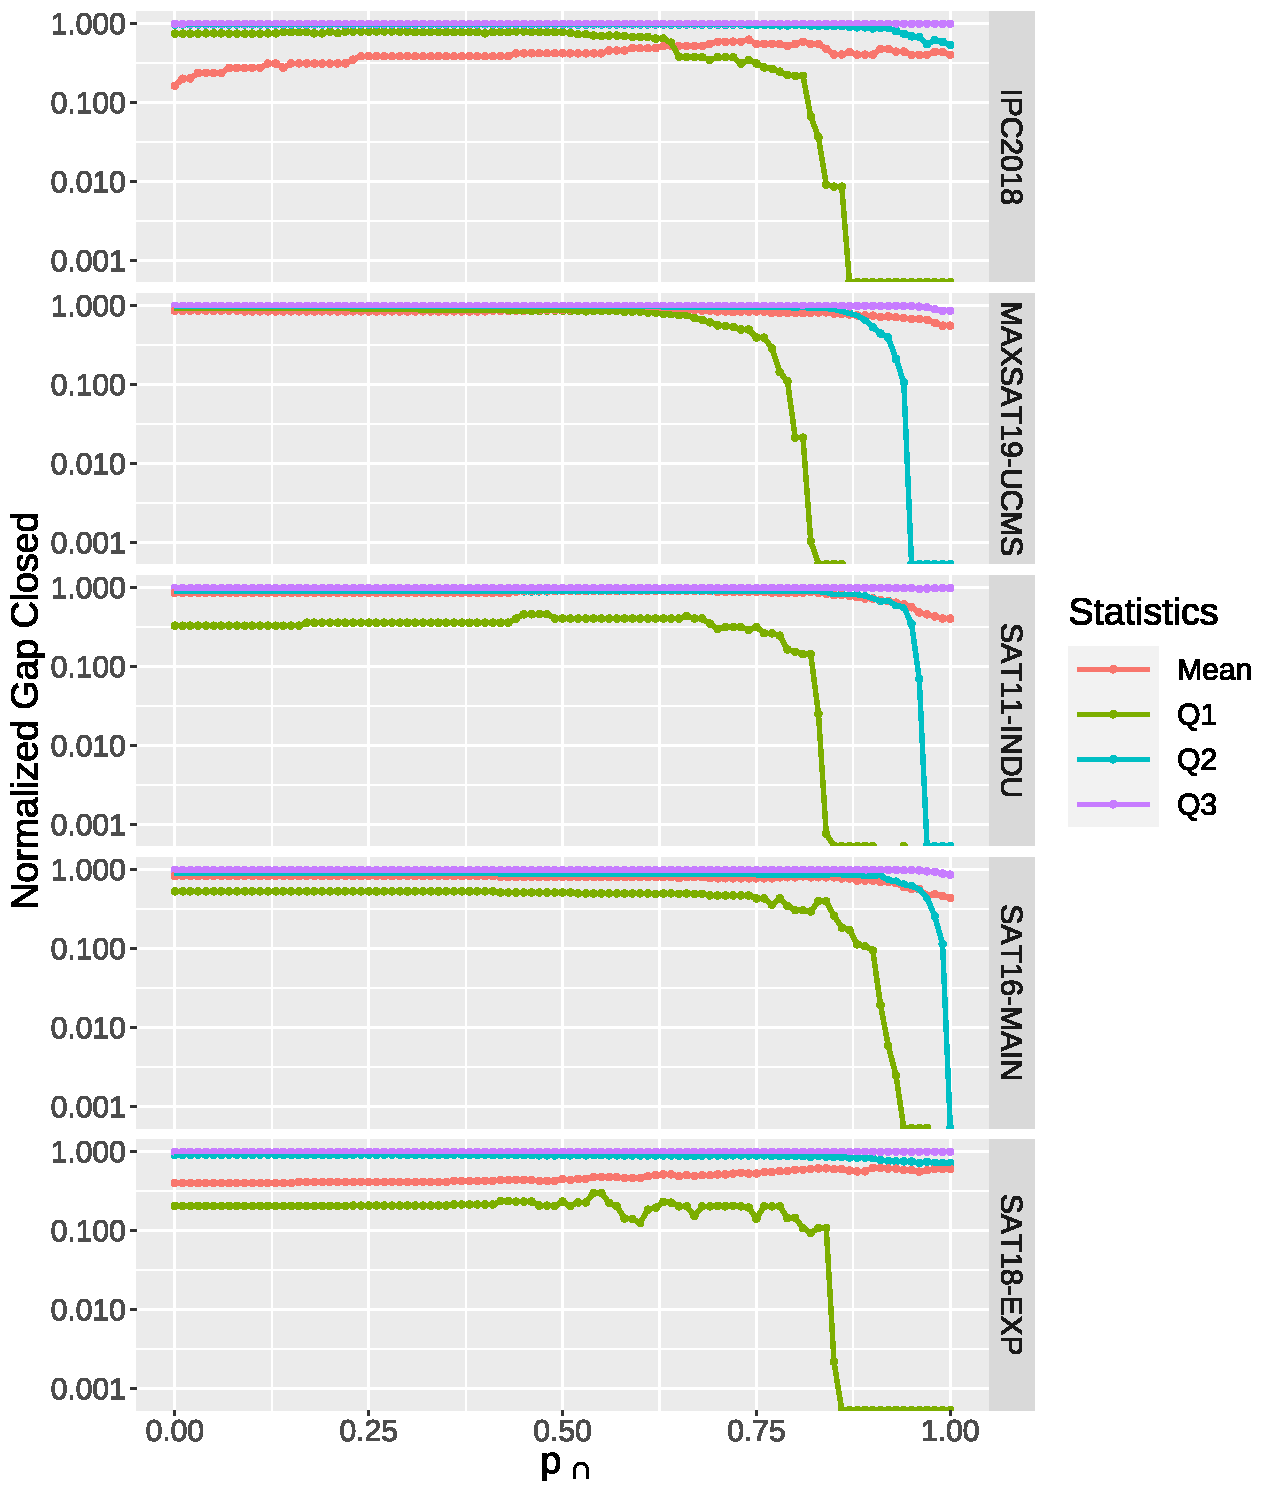
\includegraphics[width=0.48\linewidth]{plots/Theta_sensitivity_x_theta_y_runtime_facet.pdf}
    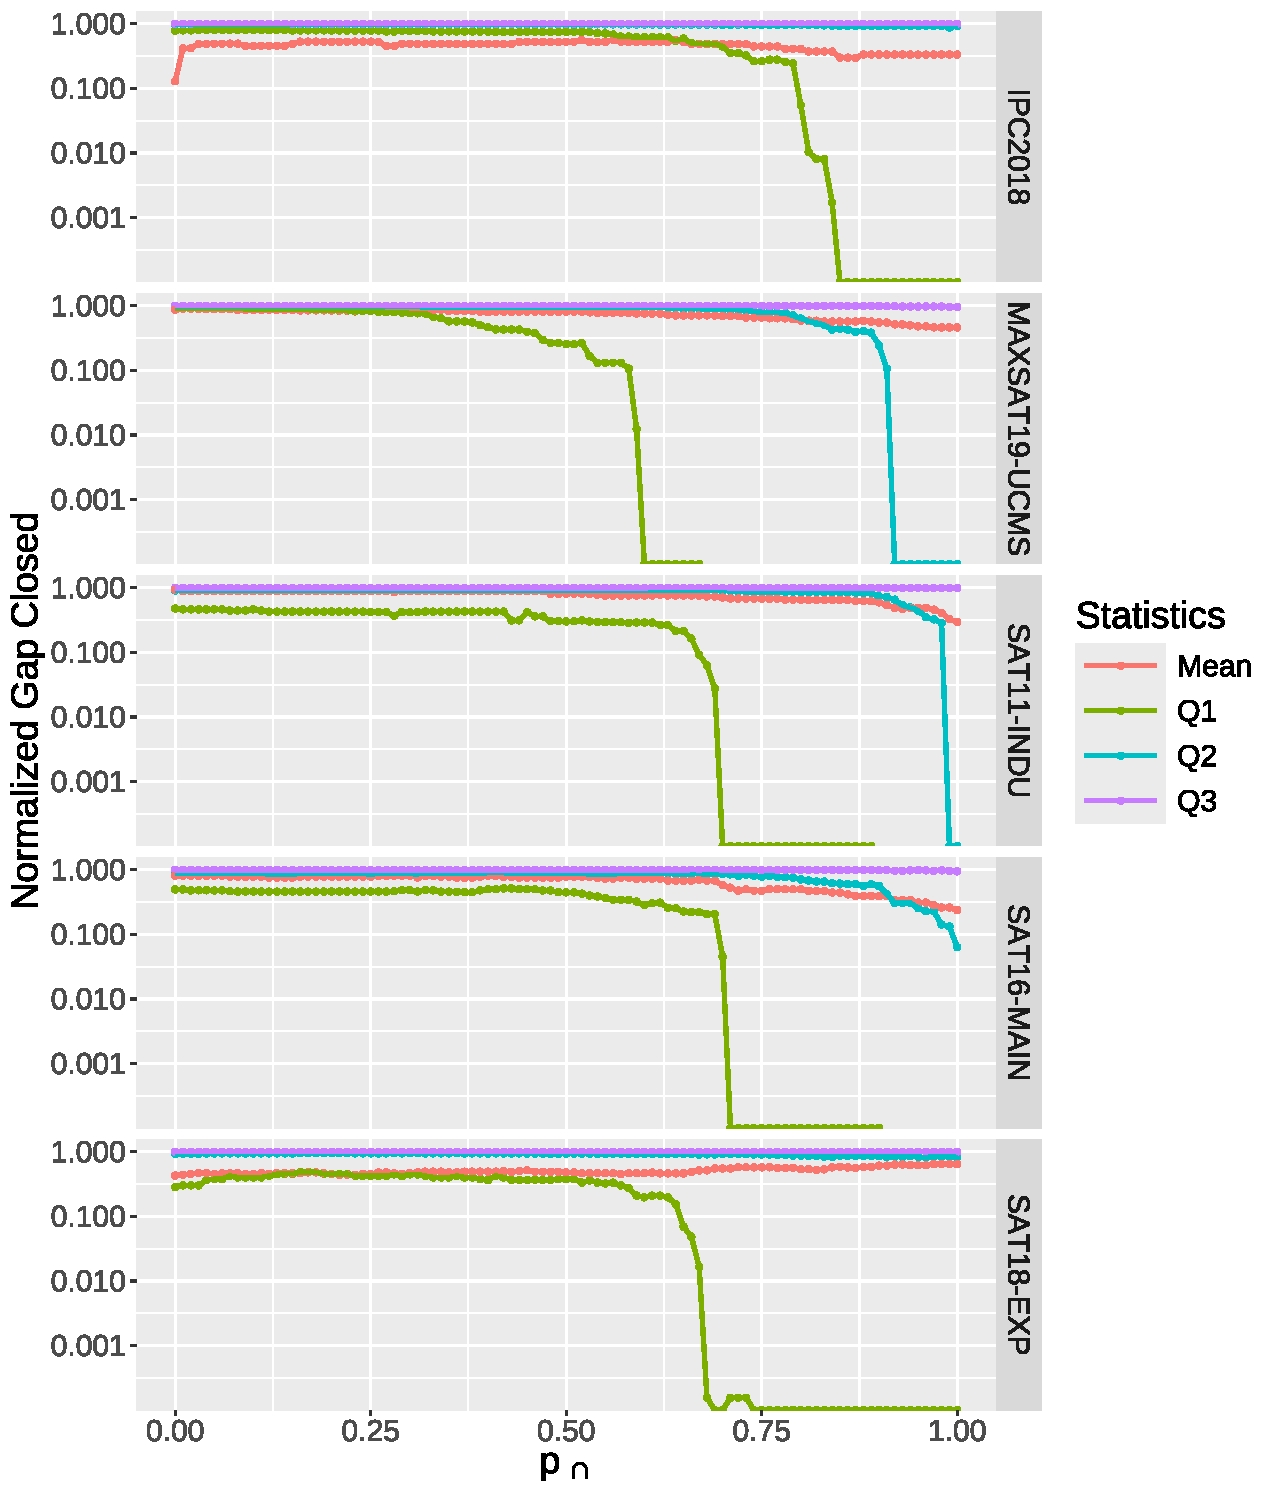
\includegraphics[width=.48\linewidth]{plots/pcap_ri_sensitivity_x_theta_y_runtime_facet.pdf}
    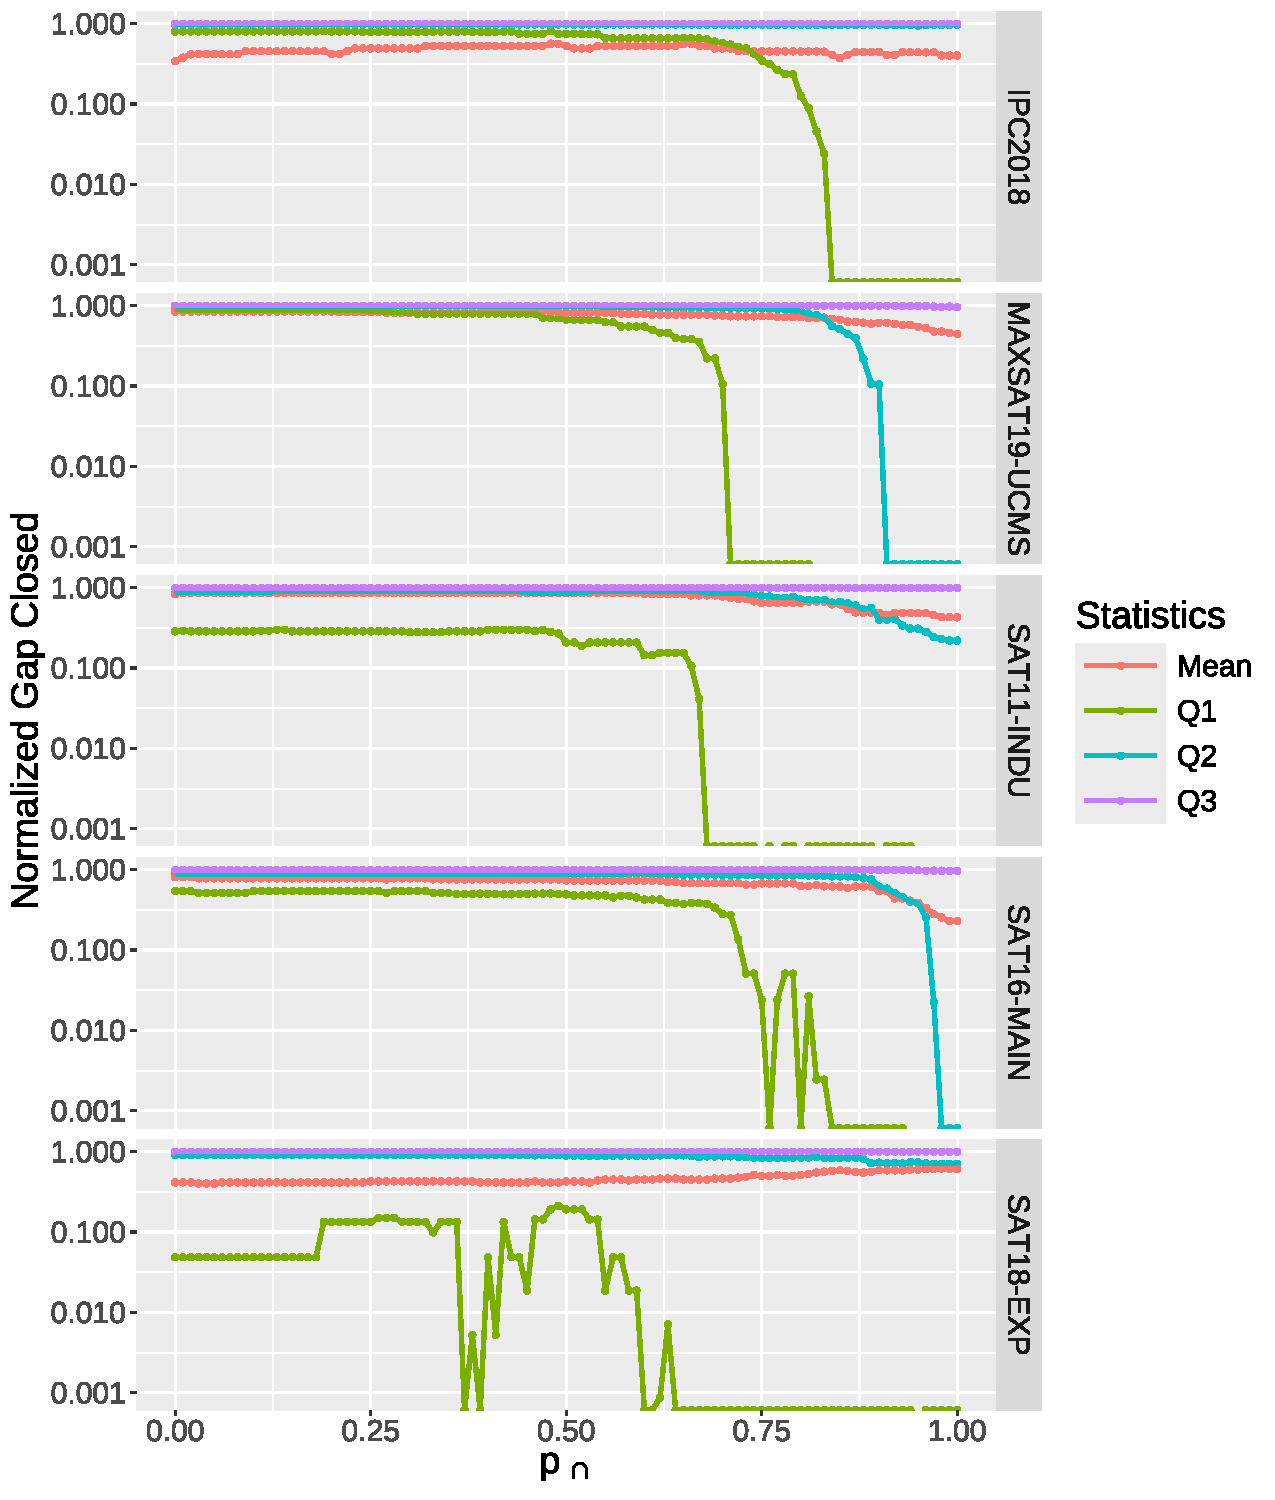
\includegraphics[width=.48\linewidth]{plots/pcap_rj_sensitivity_x_theta_y_runtime_facet.pdf}
    \caption[Sensitivity of portfolio performance to $p_{\cap}$]{Sensitivity of portfolio performance to $p_{\cap}$. The top-left plot refers to the RFJ model—Regression Random Forest model using MLR with the Jackknife uncertainty estimation method. The top-right plot refers to the RI model—Regression Ranger model with the Infinitesimal Jackknife uncertainty estimation method. The bottom plot refers to the RJ model—Regression Ranger model with the Jackknife uncertainty estimation method. The plot illustrates the mean, Q1 (25th percentile), Q2 (50th percentile), and Q3 (75th percentile) runtime performance of each scenario for various values of $p_{\cap}$ as defined in Equation~\ref{eq:7}. Note the log scale for the normalized gap closed.}
    \label{fig:sensitivity}
\end{figure}

The tuning of $p_{\cap}$ shows that the optimal value depends on the scenario. For the IPC2018 scenario, the ideal $p_{\cap}$ value is 0.59, for the MAXSAT19-UCMS scenario 0.55, for SAT11-INDU 0.63, for SAT16-MAIN 0.33, and for SAT18-EXP 0.81 for the random forest model trained using the MLR and Jackknife uncertainty estimation method (RFJ). The optimal $p_{\cap}$ values for the Ranger models, one with Jackknife (RJ) and the other with Infinitesimal Jackknife (RI), are provided in Table~\ref{tab:pcap}.

\begin{table}
\centering
\caption{Optimum value of $p_{\cap}$ for each benchmark and model.}
\label{tab:pcap}
\begin{tabular}{p{3.6cm} cccc}
\toprule
Scenario & RandomForest\_Jackknife & Ranger\_Jackknife & Ranger\_Inifinitesimal\\
\midrule
IPC2018 & 0.59 & 0.27 & 0.44 \\
MAXSAT19-UCMS & 0.55 & 0.14 & 0.03\\
SAT11-INDU & 0.63 & 0.31 & 0.01\\
SAT16-MAIN & 0.33 & 0.33 & 0\\
SAT18-EXP & 0.81 & 0.58 & 0.55\\
\midrule
Generic best & 0.82 & 0.31 & 0.17\\
\bottomrule
\end{tabular}
\end{table}


Figures~\ref{fig:sensitivity} shows the normalized gap closed for the mean, 25th percentile, 50th percentile, and 75th percentiles for each scenario depending on $p_{\cap}$. While the optimal values are very different across different scenario and each algorithm selector, the differences in terms of gap closed are relatively small as long as $p_{\cap}$ is not too large. The best average value for $p_{\cap}$ across all scenarios for RFJ model, RI model, and RJ model are 0.82, 0.17, 0.31 respectively which yields performance improvements over the baselines in most cases (see Table~\ref{tab:summary}). For the overall best performance, we recommend to tune $p_{\cap}$ for the particular scenario. However, using the generic best values of 0.82, 0.17, and 0.31 for RFJ, RI, and RJ, respectively, provides a reasonable starting point that yields good performance across the range of scenarios considered here.

The optimal value of $p_{\cap}$ allows us to draw conclusions with respect to the predictive accuracy of the performance models we are using. A small value would suggest that the predictions of the performance models are not very accurate, as we have to include even solvers whose predicted runtime distribution has a small overlap with the runtime distribution of the best predicted solver to include solvers that are actually good. If the optimal value of $p_{\cap}$ was 0, we would have to include all solvers, even the ones whose predicted distribution has no overlap with the best predicted solver -- in other words, the predicted runtime distribution of the actual best solver has no overlap with the predicted runtime distribution of the best predicted solver. 

Here, for the RFJ model, the optimal values for $p_{\cap}$ are relatively large in most cases, and even the smallest values are far greater than 0. For the RJ model, the values are lower than those for the RFJ model, except for SAT16-MAIN, where the values are equal. For the RI model, except for IPC2018, the values are even lower than those for the RJ model. This indicates that the predictions of the performance models for RFJ are quite good -- while the best predicted solver is not always the actual best solver for a given problem instance, the predicted runtime distribution of the actual best solver has a large overlap with the predicted runtime distribution of the predicted best solver. 

Based on the low values of the RI model, it appears that this model performs worse than the other two. This claim is also evident in Table~\ref{tab:summary} where, for IPC2018, MAXSAT19-UCMS, and SAT11-INDU, the performance of the $AS$ (RI) model is worse than the other two in at least two of the performance measurements. For SAT16-MAIN, the $AS$ (RI) model performs worst only in terms of PAR10, indicating more timeouts; however, on average, it provides better runtime predictions, so the runtime and MCP measures are better than those of the RJ model. For SAT18-EXP, as shown in Table~\ref{tab:pcap}, the RI model has a slightly lower $p_{\cap}$ value than the RJ model; however, the difference is minimal, and the RI model performs better than the RJ model according to Table~\ref{tab:summary}. Overall, according to Table~\ref{tab:summary}, the RFJ model outperforms the other two models in at least two performance metrics in 4 out of 5 scenarios when performing single algorithm selection.

\subsection{Algorithm Selection Results}
\begin{figure}
        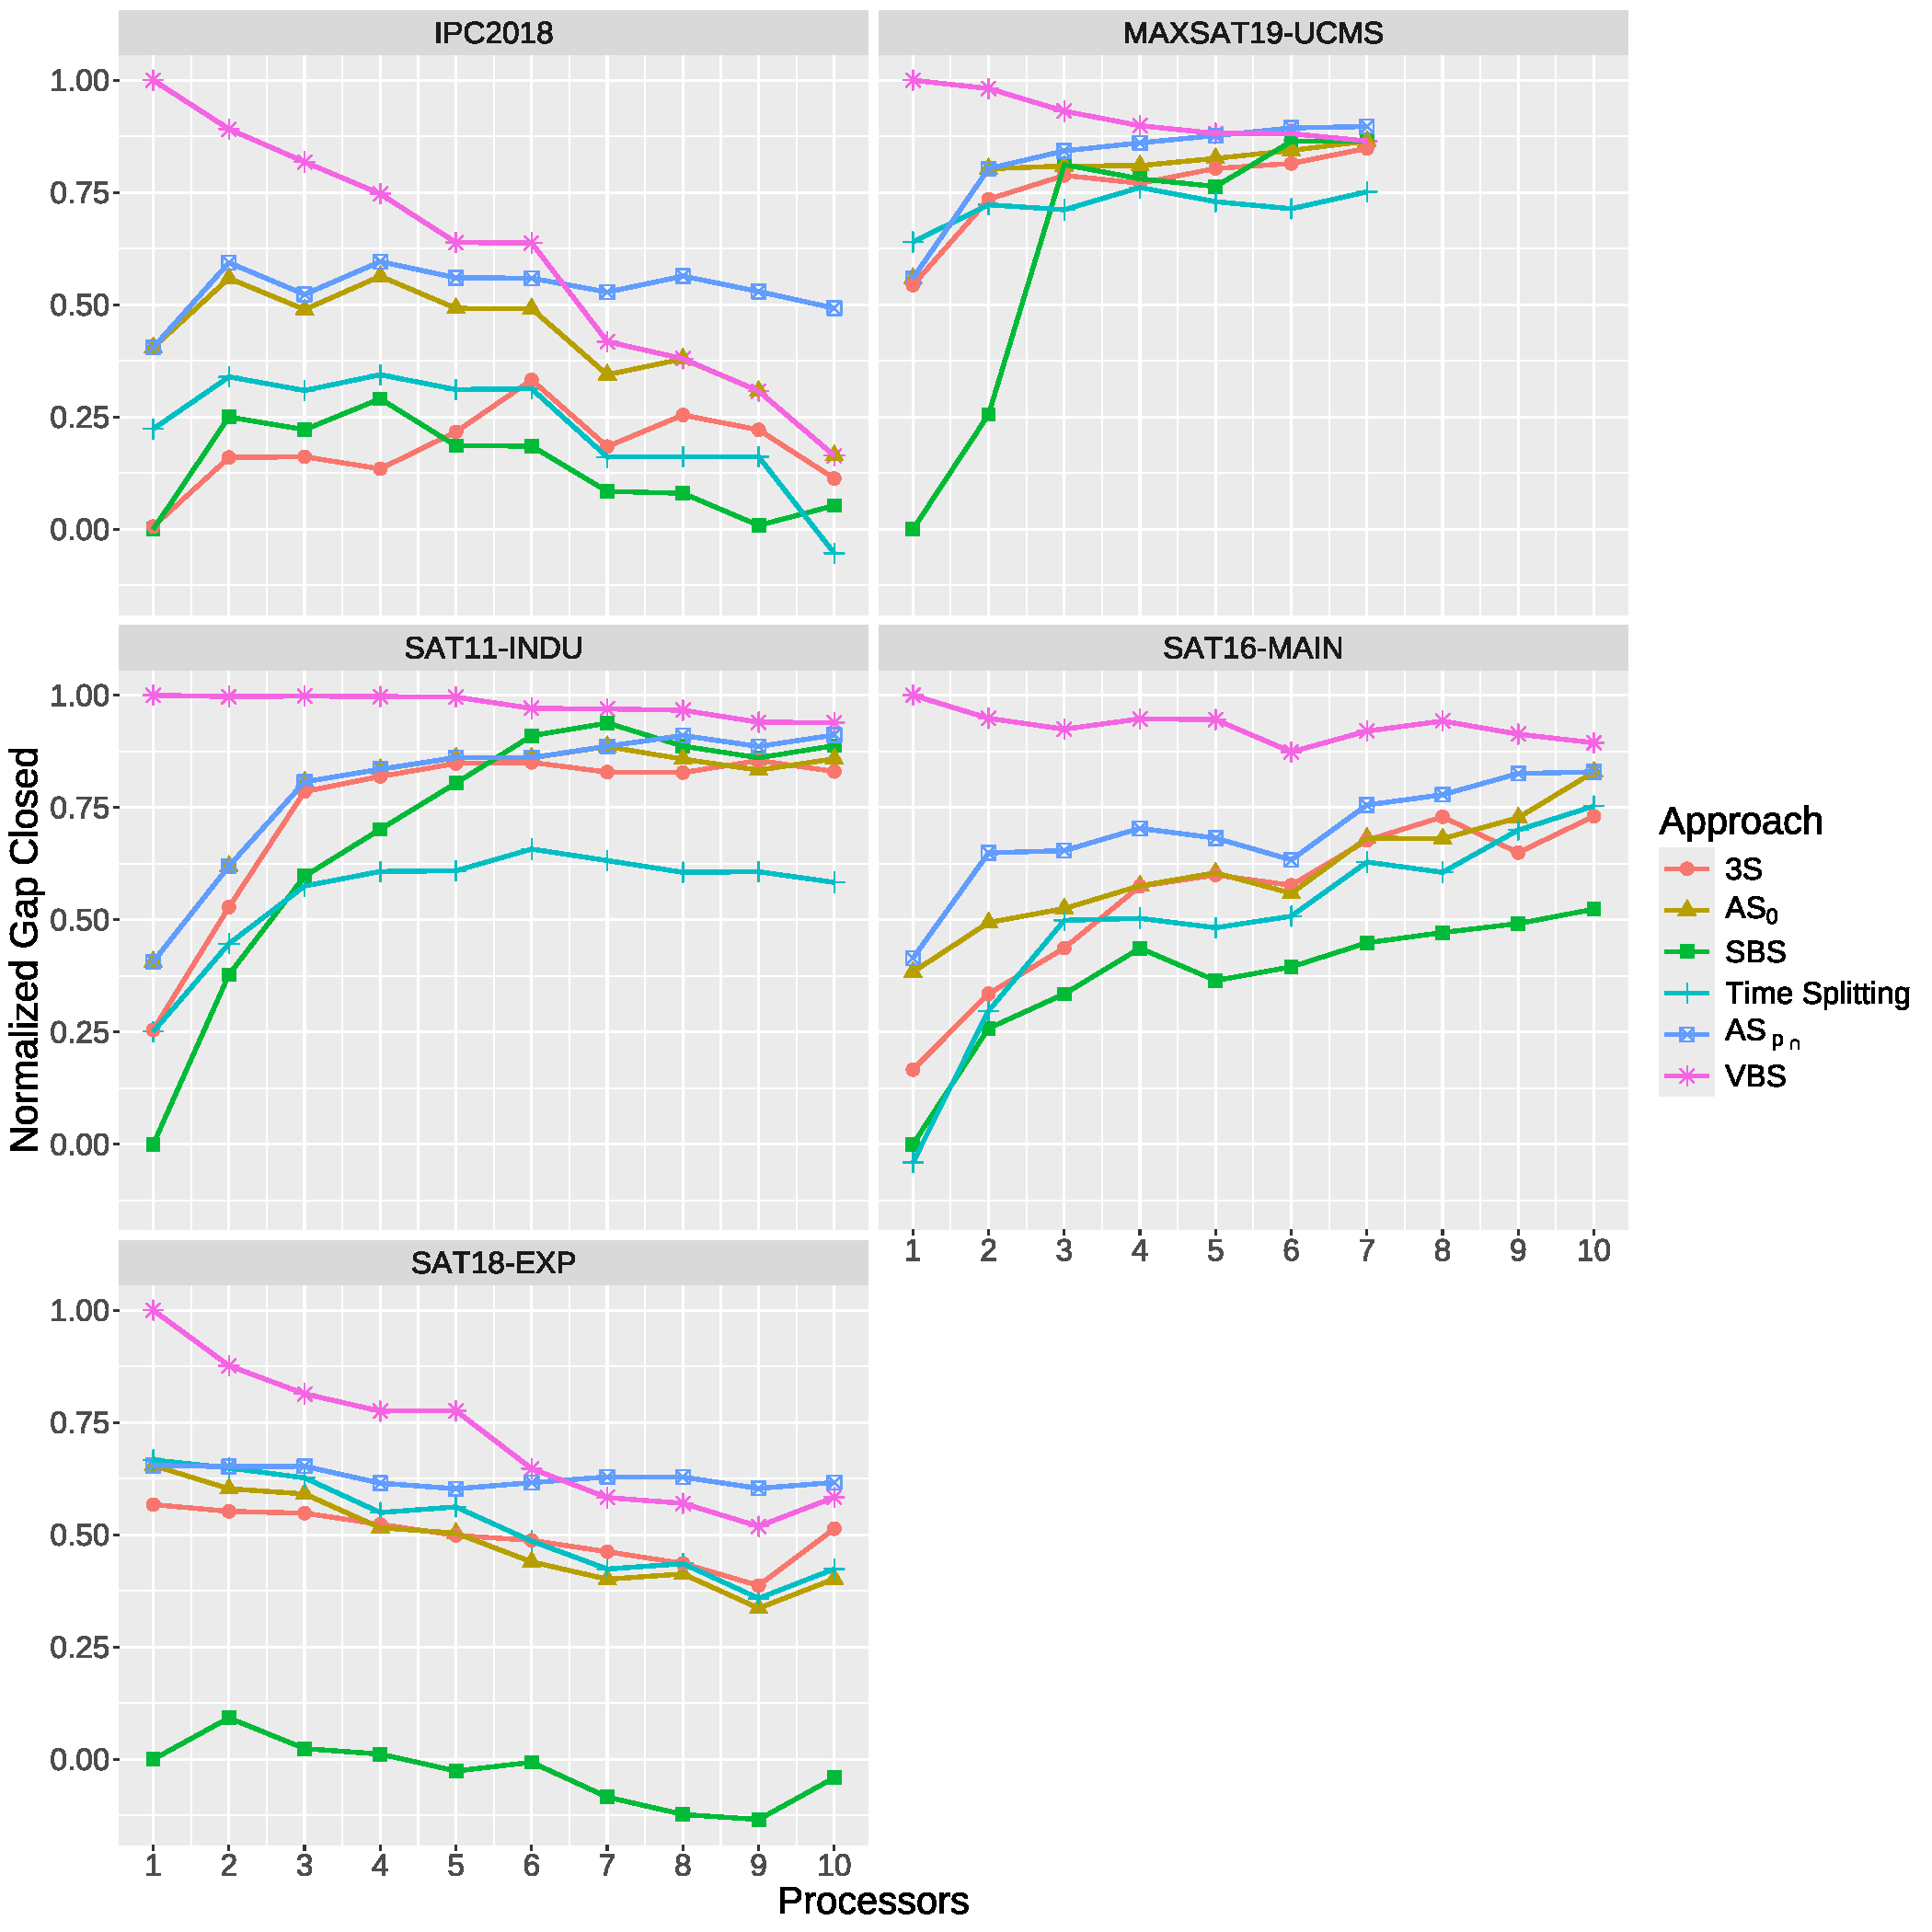
\includegraphics[width=\linewidth]{plots/line_chart_parallel_NormalizedGap_2col.pdf}    
    \caption[Results Summary: Comparing $AS_{p_{\cap}}$ with Baselines]{
    Summary of results. The plot shows the degree to which the gap between the SBS and VBS PAR10 scores is closed by each method. For the VBS and SBS, we choose the top $n$ solvers, where $n$ is the number of processors, for a given problem instance and across all instances, respectively. $AS_0$ chooses the top $n$ solvers predicted by algorithm selection, without regard for any overlap in their predicted runtime distributions. $AS_{p_{\cap}}$ represents the proposed formulation, with the number of processors restricted to at most the specific value indicated on the x axis -- depending on the overlap of the predicted runtime distributions, fewer solvers than the maximum may be chosen. The $p_{\cap}$ values for IPC2018, MAXSAT19-UCMS, SAT11-INDU, SAT18-EXP, and SAT16-MAIN are 0.59, 0.55, 0.63, 0.81, and 0.33 and respectively. Time Splitting is the baseline approach that allocates time proportional to the predicted runtime and standard deviation for each solver, scheduling more than one solver to be run per processor.}
    \label{fig:all_results}
\end{figure}

\begin{figure}
    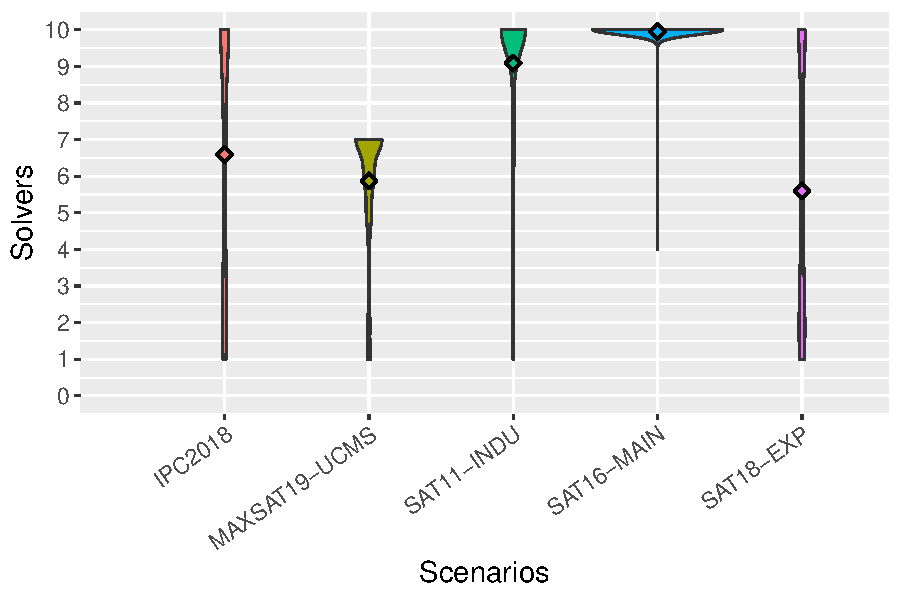
\includegraphics[width=0.5\linewidth]{plots/x_Scenario_y_Solver.pdf}
    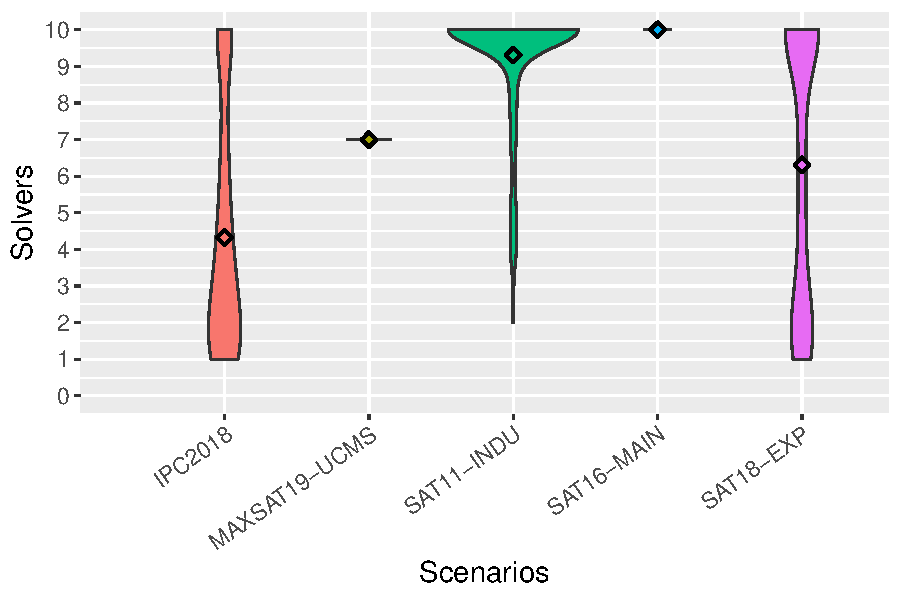
\includegraphics[width=0.5\linewidth]{plots/number_of_solvers_infjack_pcap.pdf}
    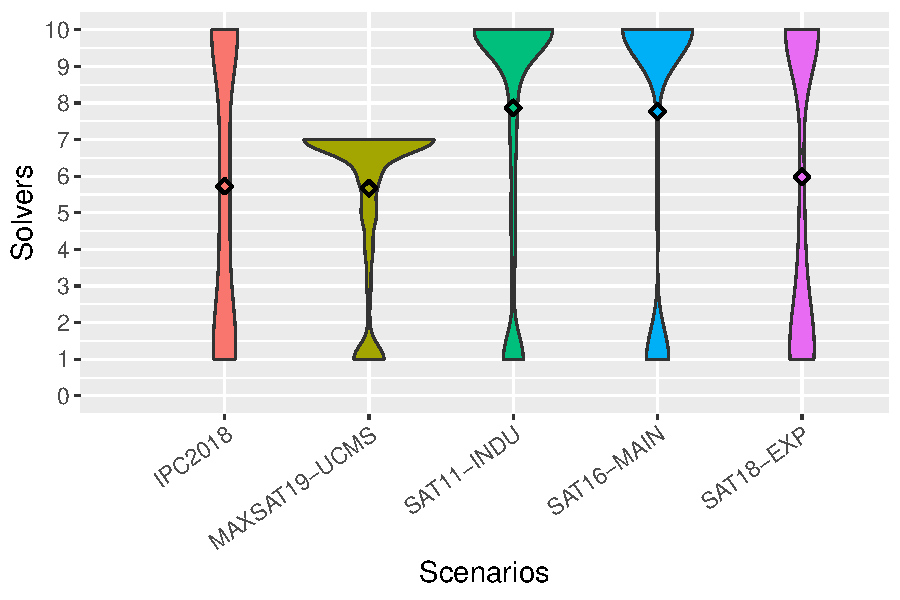
\includegraphics[width=0.5\linewidth]{plots/number_of_solvers_jack_pcap.pdf}

    \caption[Distribution of Number of Selected Solvers when Using $AS_{p_{\cap}}$]{
    Violin plot of the distribution of the number of selected solvers to run in parallel across all problem instances for each scenario for the respective optimal $p_{\cap}$ and the maximum level of parallelism (seven processors for MAXSAT19-UCMS and 10 for all other scenarios). The diamond denotes the mean value. The top-left plot refers to the RFJ model, the top-right plot to the RI model, and the bottom plot to the RJ model.
    }
    \label{fig:x_Scenario_y_Solver}
\end{figure}

To evaluate the effectiveness of our approach, we carried out a series of experiments using the optimum and the average best value for $p_{\cap}$ for each scenario using the RFJ model where we varied the number of processors used for parallel execution from one to ten for the SAT18-EXP, SAT16-MAIN, SAT11-INDU, and IPC2018 scenarios. For the MAXSAT19-UCMS scenario, we used a maximum of seven processors as there are only seven algorithms. For RFJ model Figure~\ref{fig:all_results} shows the PAR10 score results in terms of the normalized performance gap between the sequential single best solver and sequential virtual best solver for all scenarios and numbers of processors.

The figure demonstrates the promise of the approach we propose here. In three out of five scenarios, we achieve the overall top performance with the maximum number of processors (even better than the parallel virtual best solver!) and for the remaining two scenarios only the parallel virtual best solver is better. We are able to achieve better performance than the parallel virtual best solver when running in parallel because our approach does not necessarily use all available processors, unlike the baseline approaches that we compare to. While the performance of the virtual best solver suffers for a large number of parallel runs, our approach keeps the overhead of running many things in parallel low and is thus better overall. We emphasize that the results we show here are actual measured values for running in parallel, rather than assuming overhead-free parallelization based on sequential runtimes, as is commonly done in the literature. Our results demonstrate that this common assumption is unrealistic except for a small number of parallel runs.

Even for a small number of processors, our approach yields better performance than others. Initially, the performance is similar to $AS_0$ (running the top $n$ solvers), but our approach quickly becomes better as the number of available processors increases. This is expected, as for a single processor the two methods run exactly the same solver, but for a larger number of processors our method may not run as many as $AS_0$, thus decreasing overhead and overall solving performance.

For the IPC2018 scenario, we achieve the best overall results, improving performance substantially over all other approaches for 10 processors. The 3S approach is never close to the performance of our method and consistently yields worse results. The greedy time-splitting method also underperformed, often allocating time slices smaller than required to solve the instance and thus wasting resources. For more than seven parallel runs, the parallel virtual best solver, i.e.\ choosing the actual best solvers for each instance to run in parallel, starts to perform worse than our method, which does not use as many processors and incurs lower overhead.

The results for the other scenarios are qualitatively similar. While for a small number of processors, other methods perform similar to ours, the gap between them widens as the number of parallel runs increases. 3S consistently shows worse performance, whereas running the top $n$ solvers based on algorithm selection (without considering the predicted performance distributions) is usually competitive and in some cases gives the same performance as our method. The baseline of allocating a time to run proportional to the predicted runtime and standard deviation for each solver is not competitive, consistently showing bad performance -- this baseline is worse than simply running the top $n$ single best solvers in parallel on three scenarios for large numbers of parallel runs. For the IPC2018 and MAXSAT19-UCMS scenarios, the performance of some methods becomes worse than the single best solver for large numbers of processors, showing the limitations of these approaches. For the SAT2016-MAIN scenario, our approach is performing so close to the na\"ive parallel algorithm selection (top $n$ solvers based on algorithm selection) because the standard error of the predictions was large and this resulted in large parallel portfolios for the majority of instances.

Table~\ref{tab:summary} shows more detailed results. The normalized gap closed represented the mean and standard deviation of the normalized gap closed across the 10 folds, whereas the ~\ref{fig:all_results} shows the mean of the normalized gap closed across all instances at once. We see that our method results in substantial savings in terms of all three measures across all scenarios -- the proposed approach is always the best overall, regardless of the performance measure. Note that we never beat the sequential VBS, which represents the upper bound on the performance of any algorithm selection system -- we cannot do better than only running the actual best solver. In many cases, the actual performance we achieve is close to the sequential VBS though. The results also show that using the ``generic'' best value for $p_{\cap}$ of 0.82 still gives substantial performance improvements over other approaches -- usually it gives the second best performance. The only exception to this are the MAXSAT19-UCMS and SAT2016-MAIN scenarios, where running the top $n$ solvers predicted by algorithm selection does better. The gap is relatively small though, and we still beat most of the other baselines.

\begin{table}[t]
\begin{center}
    {\caption[Detailed Results: Runtime, MCP, PAR10, and Normalized Gap Closed for $AS_{p_{\cap}}$ vs. Baselines PC2018 and MAXSAT19-UCMS Scenarios]{Detailed results. Mean and standard deviation of values for runtime, MCP, and PAR10 across all problem instances in a scenario for the sequential virtual best solver, sequential single best solver, and single top predicted algorithm in the initial three rows. The second set of rows for each scenario shows the results for the maximum number of processors (10 for IPC2018, and 7 for MAXSAT19-UCMS) for our approach and the baselines we compare to. All numbers were rounded to integers. The best value for each scenario and measure is shown in \textbf{bold} (excepting the sequential VBS, which is by definition always the best), the second best in \textit{italics}. The normalized gap closed represents the mean and standard deviation of the normalized gap closed across the folds.}\label{tab:summary}}
    \scriptsize\begin{tabular}{clcccc}
    \toprule
        Scenario & Approach & Runtime [s] & MCP & PAR10 & NormalizedGap\\
    \midrule
    
    \multirow{17}{*}{\rotatebox{90}{IPC2018}} & \multicolumn{5}{c}{\textbf{1 Processor}} \\\cmidrule{2-6}
        & VBS & 508$\pm$697 & 0 & 3478$\pm$6903 & 1\\
        & AS (RFJ) & 607$\pm$751 & 99$\pm$301 & 4657$\pm$7725 & -0.44$\pm$2.84\\
        & AS (RI) & 608$\pm$751 & 100$\pm$293 & 4456$\pm$7583 & -0.35$\pm$2.85\\
        & AS (RJ) & 604$\pm$752 & 96$\pm$293 & 4519$\pm$7633 & -0.39$\pm$2.84 \\
        & SBS & 734$\pm$770 & 226$\pm$414 & 5459$\pm$8072 & 0 \\
    \cmidrule{2-6}  
    & \multicolumn{5}{c}{\textbf{10 Processors}}\\
    \cmidrule{2-6}
        %& VBS &  &  &  \\
        %& SBS &  &  & \\
        & 3S & 645$\pm$770 & 137$\pm$471 & 5235$\pm$8047 & -0.76$\pm$2.7\\
        & Time Splitting (RFJ) & 637$\pm$797 & 129$\pm$348 & 5565$\pm$8241 & -0.84$\pm$2.5\\
        & Time Splitting (RI) & 641$\pm$799 & 133$\pm$361 & 5636$\pm$8274 & -0.99$\pm$2.52\\
        & Time Splitting (RJ) & 636$\pm$794 & 128$\pm$353 & 5496$\pm$8206 &  -0.92$\pm$2.51\\
        & $AS_0$ (RFJ) & 612$\pm$779 & 104$\pm$307 & 5134$\pm$8027 & -0.66$\pm$2.56\\
        & $AS_0$ (RI)  & 616$\pm$783  & 107$\pm$312 & 5206$\pm$8065 & -0.69$\pm$2.54\\
        & $AS_0$ (RJ)  & 616$\pm$783 & 107$\pm$312 & 5206$\pm$8065 & -0.69$\pm$2.54 \\ 
        & $AS_{p_{\cap} = 0.59}$ (RFJ) & \emph{569$\pm$745} & \emph{61$\pm$223} & 4484$\pm$7651 & \textbf{-0.18$\pm$2.74} \\
        & $AS_{p_{\cap} = 0.44}$ (RI) & \textbf{557$\pm$728} & \textbf{49$\pm$190} & \textbf{4135$\pm$7403} & \emph{-0.19$\pm$2.89}\\
        & $AS_{p_{\cap} = 0.27}$ (RJ) & 570$\pm$744 & 62$\pm$229 & 4350$\pm$7552 &  -0.21$\pm$2.72 \\
        & $AS_{p_{\cap} = 0.82}$ (RFJ) & 579$\pm$742 & 70$\pm$233 & 4359$\pm$7548  & -0.26$\pm$2.88 \\
        & $AS_{p_{\cap} = 0.17}$ (RI) & 570$\pm$739 & 62$\pm$230 & \emph{4283$\pm$7501} & -0.24$\pm$2.87\\
        & $AS_{p_{\cap} = 0.31}$ (RJ) & 570$\pm$743 & 62$\pm$229 & 4350$\pm$7552 & -0.21$\pm$2.72\\
    \midrule
    \multirow{19}{*}{\rotatebox{90}{MAXSAT19-UCMS}} & \multicolumn{5}{c}{\textbf{1 Processor}} \\\cmidrule{2-6}
        & VBS & 858$\pm$1476 & 0 & 7768$\pm$14717 & 1\\
        & AS (RFJ) & 1037$\pm$1555 & 179$\pm$641 & 9363$\pm$15684 & 0.55$\pm$0.28\\
        & AS (RI) & 1076$\pm$1575 & 218$\pm$729 & 9686$\pm$15850 & 0.45$\pm$0.34 \\
        & AS (RJ) & 1044$\pm$1565 & 186$\pm$666 & 9540$\pm$15793 & 0.49$\pm$0.23 \\
        & SBS & 1190$\pm$1657 & 332$\pm$940 & 11386$\pm$16696 & 0 \\
    \cmidrule{2-6}   
    & \multicolumn{5}{c}{\textbf{7 Processors}}\\
    \cmidrule{2-6}  
        %& VBS & 894.42 & 37.11 & 8258.05 \\
        %& SBS & 894.42 & 37.11 & 8258.05\\
        & 3S & 953$\pm$1480 & 95$\pm$437 & 8317$\pm$15031 & 0.83$\pm$0.16 \\
        & Time Splitting (RFJ) & 908$\pm$1523 & 51$\pm$308 & 8668$\pm$15353 & 0.75$\pm$0.16 \\
        & Time Splitting (RI) & 919$\pm$1535 & 61$\pm$356 & 8849$\pm$15470  & 0.7$\pm$0.2\\
        & Time Splitting (RJ) & 917$\pm$1531 & 59$\pm$352 & 8790$\pm$15431 & 0.71$\pm$0.2 \\
        & $AS_0$ (RFJ) & \emph{894$\pm$1506} & \emph{37$\pm$247} & 8258$\pm$15062 & 0.85$\pm$0.16\\
        & $AS_0$ (RI) & \emph{894$\pm$1506} & \emph{37$\pm$247} & 8258$\pm$15062 & 0.85$\pm$0.16 \\ 
        & $AS_0$ (RJ) & \emph{894$\pm$1506} & \emph{37$\pm$247} & 8258$\pm$15062 & 0.85$\pm$0.16\\
        & $AS_{p_{\cap} = {0.55}}$ (RFJ) & \textbf{891$\pm$1496} & \textbf{33$\pm$215} & \textbf{8141$\pm$14975} & \textbf{0.88$\pm$0.17} \\
        & $AS_{p_{\cap} = 0.03}$ (RI) & \emph{894$\pm$1506} & \emph{37$\pm$247} & 8258$\pm$15062 & 0.85$\pm$0.16  \\ 
        & $AS_{p_{\cap} = 0.14}$ (RJ) & 921$\pm$1521 & 63$\pm$369 & 8568$\pm$15263 &  0.76$\pm$0.24 \\
        & $AS_{p_{\cap} = 0.82}$ (RFJ) & 928$\pm$1513 & 70$\pm$364 & 8461$\pm$15175 & 0.81$\pm$0.18\\
        & $AS_{p_{\cap} = 0.17}$ (RI) & 901$\pm$1502 & 43$\pm$275 & \emph{8208$\pm$15015} &  \textbf{0.88$\pm$0.16} \\
        & $AS_{p_{\cap} = 0.31}$ (RJ) & 931$\pm$1525 & 73$\pm$402 & 8578$\pm$15259 & 0.78$\pm$0.21 \\
\bottomrule
    \end{tabular}    
\end{center}
\end{table}


\begin{table}[t]
\begin{center}
    {\caption[Detailed Results: Runtime, MCP, PAR10, and Normalized Gap Closed for $AS_{p_{\cap}}$ vs. Baselines for SAT11-INDU and SAT16-MAIN Scenar]{Detailed results. Mean and standard deviation of values for runtime, MCP, and PAR10 across all problem instances in a scenario for the sequential virtual best solver, sequential single best solver, and single top predicted algorithm in the initial three rows. The second set of rows for each scenario shows the results for the maximum number of processors (10 for SAT16-MAIN and SAT11-INDU) for our approach and the baselines we compare to. All numbers were rounded to integers. The best value for each scenario and measure is shown in \textbf{bold} (excepting the sequential VBS, which is by definition always the best), the second best in \textit{italics}. The normalized gap closed represents the mean and standard deviation of the normalized gap closed across the folds.}\label{tab:summary2}}
    \scriptsize\begin{tabular}{clcccc}
    \toprule
        Scenario & Approach & Runtime [s] & MCP & PAR10 & NormalizedGap\\
    \midrule
    \multirow{17}{*}{\rotatebox{90}{SAT11-INDU}} & \multicolumn{5}{c}{\textbf{1 Processor}} \\\cmidrule{2-6}
        & VBS & 1140$\pm$1836 & 0 & 8040$\pm$17905 & 1\\
        & AS (RFJ) & 1535$\pm$2058 & 395$\pm$1037 & 11735$\pm$20768 & 0.16$\pm$0.79\\        
        & AS (RI) & 1610$\pm$2108 & 470$\pm$1145 & 12710$\pm$21389 & -0.06$\pm$0.9\\
        & AS (RJ) & 1565$\pm$2049 & 425$\pm$1017 & 11315$\pm$20402 & 0.34$\pm$0.49\\
        & SBS & 1818$\pm$2168 & 678$\pm$1340 & 14268$\pm$22154 & 0 \\
    \cmidrule{2-6}    
    & \multicolumn{5}{c}{\textbf{10 Processors}}\\
    \cmidrule{2-6}    
        %& VBS &  &  &  \\
        %& SBS &  &  &  \\
        & 3S & 1298$\pm$1898 & 158$\pm$546 & 9098$\pm$18780 & 0.78$\pm$0.3\\
        & Time Splitting (RFJ) & 1335$\pm$2009 &  225$\pm$708 & 10635$\pm$20138 & 0.49$\pm$0.61 \\
        & Time Splitting (RI) & 1429$\pm$2108 & 318$\pm$875 & 12379$\pm$21378 & 0.19$\pm$0.53\\
        & Time Splitting (RJ) & 1334$\pm$1998 & 224$\pm$689 & 10634$\pm$20138 & 0.55$\pm$0.43 \\
        & $AS_0$ (RFJ) & 1272$\pm$1927 & 161$\pm$548 & 8922$\pm$18645 & \emph{0.89$\pm$0.12}\\
        & $AS_0$ (RI) & \emph{1238$\pm$1892} & 127$\pm$385 & \emph{8588$\pm$18350} & \textbf{0.92$\pm$0.1}\\ 
        & $AS_0$ (RJ) & 1262$\pm$1910 & 151$\pm$480 & 8612$\pm$18342 & \textbf{0.92$\pm$0.1} \\
        & $AS_{p_{\cap} = 0.63}$ (RFJ) & 1241$\pm$1901 & 131$\pm$451 & 8591$\pm$18349 & \textbf{0.92$\pm$0.1} \\
        & $AS_{p_{\cap} = 0.01}$ (RI) & \textbf{1236$\pm$1890} & \textbf{121$\pm$379} & \textbf{8586$\pm$18351} & \textbf{0.92$\pm$0.1} \\ 
        & $AS_{p_{\cap} = 0.31}$ (RJ) & 1289$\pm$1934 & 178$\pm$595 & 9089$\pm$18787 & 0.78$\pm$0.28\\
        & $AS_{p_{\cap} = 0.82}$ (RFJ) & 1247$\pm$1900 & \emph{123$\pm$431} & 8747$\pm$18501 &  0.83$\pm$0.28 \\
        & $AS_{p_{\cap} = 0.17}$ (RI) & 1259$\pm$1912 & 139$\pm$477 & 8909$\pm$18649 & 0.74$\pm$0.36\\
        & $AS_{p_{\cap} = 0.31}$ (RJ) & 1289$\pm$1934 & 178$\pm$595 & 9089$\pm$18787 & 0.78$\pm$0.28 \\
    \midrule 
    \multirow{19}{*}{\rotatebox{90}{SAT16-MAIN }} & \multicolumn{5}{c}{\textbf{1 Processor}} \\\cmidrule{2-6}
        & VBS & 1867$\pm$2193 & 0 & 15005$\pm$22530 & 1\\
        & AS (RFJ) & 2315$\pm$2273 & 448$\pm$1109 & 19066$\pm$23883 & 0.33$\pm$0.56\\
        & AS (RI) & 2383$\pm$2294 & 516$\pm$1151 & 19956$\pm$24111 & 0.05$\pm$0.66\\ 
        & AS (RJ) & 2400$\pm$2269 & 533$\pm$1177 & 19316$\pm$23880 & 0.3$\pm$0.24\\ 
        & SBS & 2560$\pm$2294 & 693$\pm$1415 & 21940$\pm$24464 & 0\\
    \cmidrule{2-6}
    & \multicolumn{5}{c}{\textbf{10 Processors}}\\
    \cmidrule{2-6}
        %& VBS &  1944.82 & 78.13 & 15740.44\\
        %& SBS & 2214.08 & 347.38 & 18308.97\\
        & 3S & 2093$\pm$2228 & 226$\pm$547 & 16874$\pm$23228 & 0.59$\pm$0.59\\
        & Time Splitting (RFJ) & 2101$\pm$2247 & 234$\pm$732 & 16717$\pm$23149 & \textbf{0.78$\pm$0.46} \\
        & Time Splitting (RI) & 2089$\pm$2256 & 222$\pm$642 & 17691$\pm$23593 & 0.37$\pm$0.85\\
        & Time Splitting (RJ) & 2098$\pm$2254 & 231$\pm$674 & 17372$\pm$23447 & 0.56$\pm$0.39\\
        & $AS_0$ (RFJ) & 2065$\pm$2221 & 198$\pm$652 & \textbf{16189$\pm$22931} & \emph{0.7$\pm$0.39}\\
        & $AS_0$ (RI)& \textbf{2016$\pm$2225} & \textbf{150$\pm$503} & 16469$\pm$23122 & 0.68$\pm$0.6\\ 
        & $AS_0$ (RJ)& 2048$\pm$2228 & 181$\pm$597 & \emph{16336$\pm$23023} & 0.68$\pm$0.59\\ 
        & $AS_{p_{\cap} = 0.33}$ (RFJ) & 2065$\pm$2221 & 198$\pm$652 & \textbf{16189$\pm$22931} & \emph{0.7$\pm$0.39}\\
        & $AS_{p_{\cap} = 0}$ (RI) & \textbf{2016$\pm$2225} & \textbf{150$\pm$503} & 16469$\pm$23122 & 0.68$\pm$0.6\\ 
        & $AS_{p_{\cap} = 0.33}$ (RJ) & 2088$\pm$2239 & 222$\pm$704  & 16705$\pm$23156 & 0.64$\pm$0.37\\ 
        & $AS_{p_{\cap} = 0.82}$ (RFJ) & 2094$\pm$2222 & 228$\pm$730 & 16383$\pm$22993 & 0.69$\pm$0.41\\
        & $AS_{p_{\cap} = 0.17}$ (RI) & \emph{2041$\pm$2230} & \emph{174$\pm$591} & 16822$\pm$23261 & 0.57$\pm$0.63\\
        & $AS_{p_{\cap} = 0.31}$ (RJ) & 2096$\pm$2240 & 229$\pm$713 & 16877$\pm$23227 & 0.63$\pm$0.36\\  
        \bottomrule
    \end{tabular}    
\end{center}
\end{table}
\begin{table}[t]
\begin{center}
    {\caption[Detailed Results: Runtime, MCP, PAR10, and Normalized Gap Closed for $AS_{p_{\cap}}$ vs. Baselines for SAT18-EXP Scenario]{Detailed results. Mean and standard deviation of values for runtime, MCP, and PAR10 across all problem instances in a scenario for the sequential virtual best solver, sequential single best solver, and single top predicted algorithm in the initial three rows. The second set of rows for each scenario shows the results for the maximum number of processors (10 for SAT18-EXP) for our approach and the baselines we compare to. All numbers were rounded to integers. The best value for each scenario and measure is shown in \textbf{bold} (excepting the sequential VBS, which is by definition always the best), the second best in \textit{italics}. The normalized gap closed represents the mean and standard deviation of the normalized gap closed across the folds.}\label{tab:summary3}}
    \scriptsize\begin{tabular}{clcccc}
    \toprule
        Scenario & Approach & Runtime [s] & MCP & PAR10 & NormalizedGap\\
    \midrule    
    \multirow{19}{*}{\rotatebox{90}{SAT18-EXP }} & \multicolumn{5}{c}{\textbf{1 Processor}} \\\cmidrule{2-6}
         & VBS & 1146$\pm$1945 & 0 & 9687$\pm$19547 & 1\\
         & AS (RFJ) & 1615$\pm$2138 & 468$\pm$1192 & 13470$\pm$21889 & 0.64$\pm$0.18\\
         & AS (RI) & 1648$\pm$2151 & 502$\pm$1256 & 13758$\pm$22034 & 0.59$\pm$0.18\\
         & AS (RJ) & 1690$\pm$2170 & 543$\pm$1302 & 14183$\pm$22247 & 0.57$\pm$0.16\\
         & SBS & 2400$\pm$2249 & 1254$\pm$1832 & 20629$\pm$24280 & 0\\
    \cmidrule{2-6}    
    & \multicolumn{5}{c}{\textbf{10 Processors}}\\
    \cmidrule{2-6}    
         %& VBS & 1496.22 & 350.06 & 14244.10 \\
         %& SBS & 2210.87 & 1064.70 & 21077.73 \\
         & 3S & 1625$\pm$2228 & 479$\pm$1265 & 15010$\pm$22802 & 0.5$\pm$0.23\\
         & Time Splitting (RFJ) & 1714$\pm$2292 & 571$\pm$1384 & 15992$\pm$23222 & 0.42$\pm$0.23\\
         & Time Splitting (RI) & 1640$\pm$2266 & 497$\pm$1280 & 15408$\pm$23003 & 0.46$\pm$0.24\\
         & Time Splitting (RJ) & 1745$\pm$2308  & 602$\pm$1434 & 16151$\pm$23267 & 0.4$\pm$0.24\\
         & $AS_0$ (RFJ) & 1702$\pm$2301 & 559$\pm$1389 & 16235$\pm$23355 & 0.39$\pm$0.27\\
         & $AS_0$ (RI) & 1654$\pm$2285 & 511$\pm$1324 & 15804$\pm$23194 & 0.42$\pm$0.29\\
         & $AS_0$ (RJ) & 1678$\pm$2288 & 535$\pm$1351 & 15956$\pm$23243 & 0.4$\pm$0.3 \\
         & $AS_{p_{\cap} = 0.81}$ (RFJ) & \textbf{1518$\pm$2172} & \textbf{372$\pm$1124} & \textbf{13884$\pm$22265} & \textbf{0.62$\pm$0.22} \\
         & $AS_{p_{\cap} = 0.55}$ (RI) & 1541$\pm$2191 & 397$\pm$1177 & 14034$\pm$22332 & \emph{0.6$\pm$0.21}\\ 
         & $AS_{p_{\cap} = 0.58}$ (RJ) & 1622$\pm$2237 & 477$\pm$1268 & 15008$\pm$22805 & 0.5$\pm$0.25\\
         & $AS_{p_{\cap} = 0.82}$ (RFJ) & \emph{1532$\pm$2178} & \emph{386$\pm$1146} &  \emph{14025$\pm$22336} & \emph{0.6$\pm$0.23}\\
         & $AS_{p_{\cap} = 0.17}$ (RI) & 1555$\pm$2221 & 410$\pm$1191 & 14558$\pm$22628 & 0.57$\pm$0.23\\
         & $AS_{p_{\cap} = 0.31}$ (RJ) & 1649$\pm$2265 & 505$\pm$1319 & 15544$\pm$23064 & 0.46$\pm$0.26\\
    \bottomrule
    \end{tabular}    
\end{center}
\end{table}
\subsection{Number of Selected Solvers}

As mentioned above, allowing our approach to use up to a certain number of processors does not mean that this exact number of parallel runs will be done. In practice, it is often much lower than that, as we see when comparing the performance of our approach to $AS_0$, which runs the top $n$ predicted solvers in parallel. Figure~\ref{fig:x_Scenario_y_Solver} shows the distribution of the number of selected solvers for each scenario and each algorithm selector. For RFJ, the mean number of solvers chosen for IPC2018 is around 6.5, for MAXSAT19-UCMS around 6 (out of 7), for SAT11-INDU around 9, for SAT16-MAIN around 10, and for SAT18-EXP around 5.5. For RI, the mean number of solvers chosen for IPC2018 is around 4.5, for MAXSAT19-UCMS around 7 (out of 7), for SAT11-INDU around 9.5, for SAT16-MAIN around 10, and for SAT18-EXP around 6.5. Similarly, for RJ, the mean number of solvers chosen for IPC2018 is around 6, for MAXSAT19-UCMS around 6 (out of 7), for SAT11-INDU around 8, for SAT16-MAIN around 8, and for SAT18-EXP around 6. 

For RFJ, we see that the largest difference to the maximum number of parallel runs occurs for the two scenarios where we observe the largest performance improvements of our approach, IPC2018 and SAT18-EXP. Similarly, the scenario with the highest number of solvers chosen on average (SAT16-MAIN) is where we see the smallest performance improvement. For RI and RJ the same comparison also exists. This clearly shows again that the advantage of our approach is that it does not simply use as many parallel processors as are available, which increases overhead, but intelligently chooses how many of the available processors to use for best performance. In at least some cases, more is less, and we show how to leverage this.

Figure~\ref{fig:x_Scenario_y_Solver} also shows that our approach uses the full range of available parallel runs in most cases, from running only a single solver to as many parallel runs as there are processors. Our approach is not simply a one-size-fits all that usually uses a similar number of runs, but varies the size of the selected parallel portfolio dynamically, based on the instance to be solved.

\subsection{Ranger vs RandomForest Results}
Figure~\ref{fig:rangervsrf} presents a comparison between the random forest implementation and the ranger implementations. When comparing the naive algorithm selection methods $AS (RFJ)$, $AS (RJ)$ and $AS (RI)$, which select the best predicted algorithm, based on Tables~\ref{tab:summary},~\ref{tab:summary2} and~\ref{tab:summary3}, the RFJ model emerges as a more promising algorithm selector in all scenarios except IPC2018, where the RJ model performs slightly better in terms of runtime and MCP. For SAT11-INDU, the $AS (RFJ)$ method is superior in terms of runtime and MCP, but performs slightly worse than the RI model in terms of PAR10.

When we compare $AS_{0} (RFJ)$, $AS_{0} (RJ)$, and $AS_{0} (RI)$, which select the top predicted algorithms to run in parallel, the performance of these methods is very competitive. In some cases, the RI model performs better, such as in SAT18-EXP and SAT11-INDU, across all metrics, and is superior only in terms of runtime and MCP in SAT16-MAIN. In other cases, the RFJ model performs better, as seen in IPC2018. For MAXSAT19-UCMS, all algorithm selectors perform equally, as with $p_{\cap} = 0$, all 7 available solvers are selected.

When comparing the methods using a tuned value of $p_{\cap}$, denoted as $AS_{p_{\cap}}$, the RI model outperformed the others in most cases. In IPC2018 and SAT11-INDU, it was superior in terms of runtime, MCP, and PAR10. For SAT16-MAIN, it outperformed the other two in terms of MCP and runtime, although the PAR10 of RFJ was slightly better. For MAXSAT19-UCMS and SAT18-EXP, the RFJ model performed better than the others across all performance metrics. It is worth mentioning that the RJ model could not beat other models in the $AS_{p_{\cap}}$ method. 

These comparisons is based on the runtime, MCP, and PAR10 scores listed in Tables~\ref{tab:summary}, \ref{tab:summary2}, and \ref{tab:summary3}. As shown in Figure~\ref{fig:rangervsrf}, a similar comparison exists, with the values representing the PAR10 score normalized gap closed between SBS and VBS. In this context, $AS_{p_{\cap}} (RI)$ is superior in three out of five scenarios, while $AS_{p_{\cap}} (RFJ)$ performs best in the remaining two scenarios. Although using RI for single algorithm selection performed the worst, it appears to be a better model for applying the portfolio selection approach. 

\begin{figure}[t]
        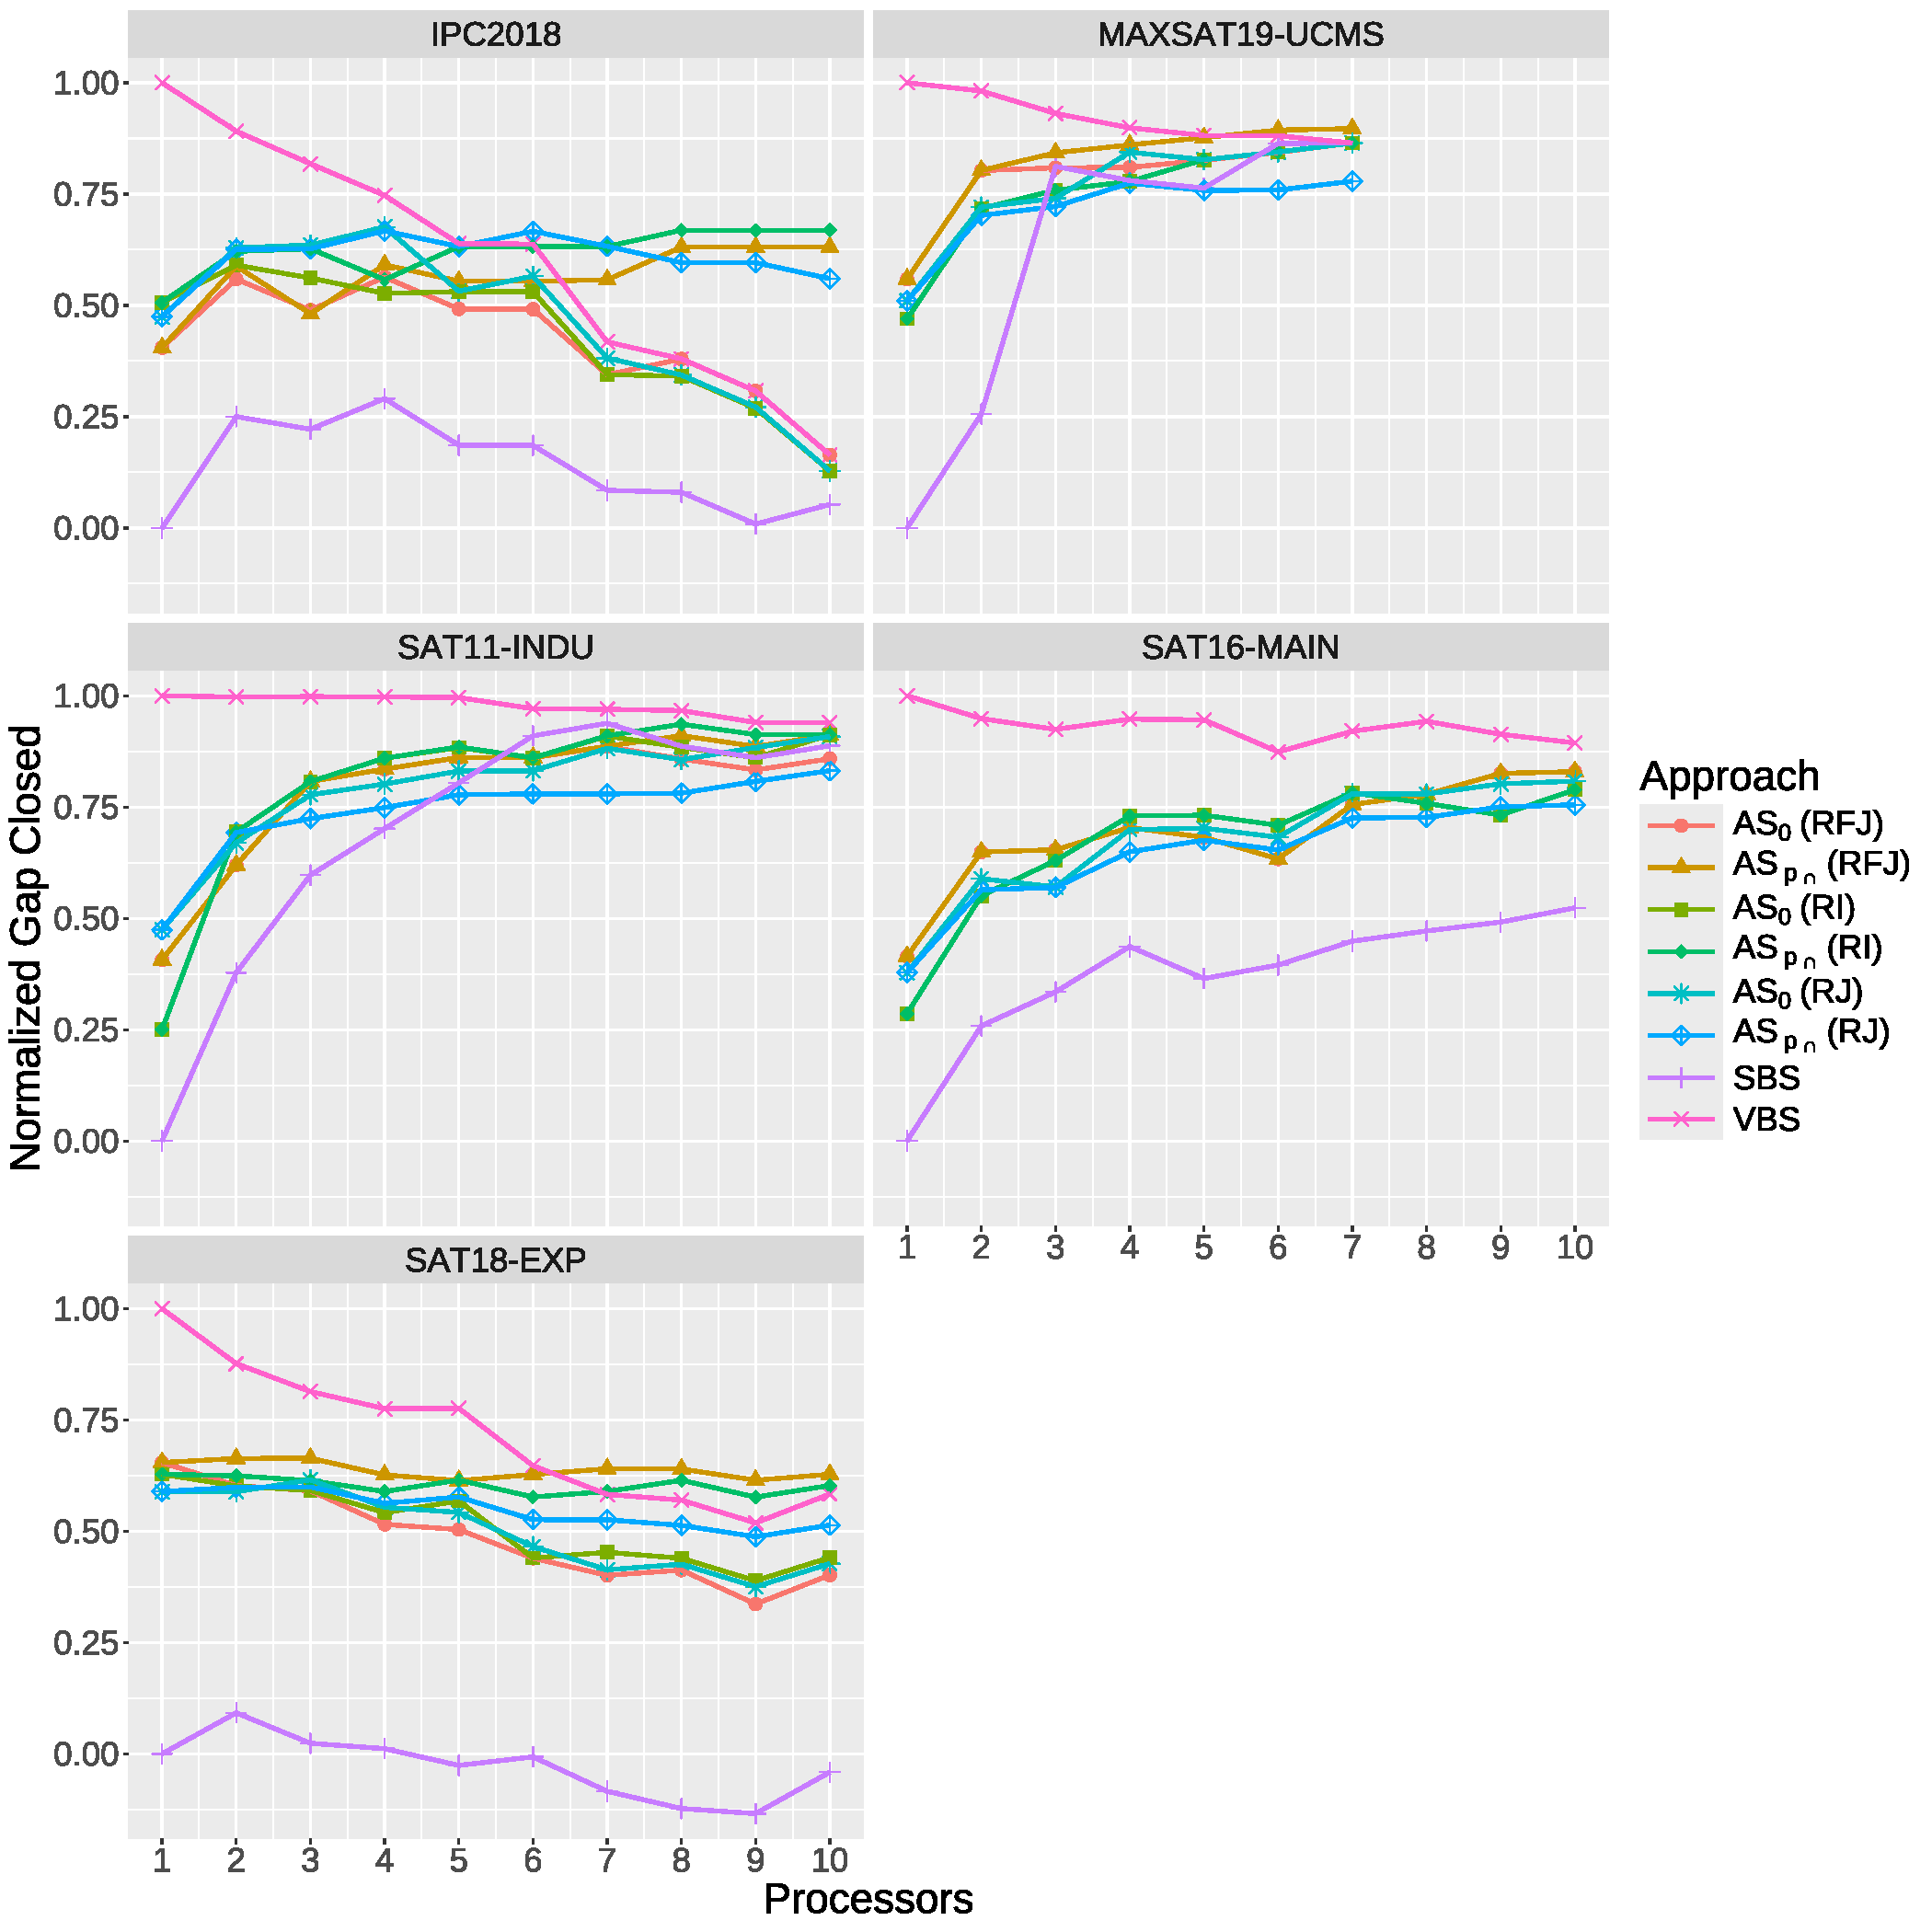
\includegraphics[width=\linewidth]{plots/learner_comparison_line_chart_parallel_NormalizedGap.pdf}    
    \caption[Results Summary: Comparing Ranger and RandomForest Models in $AS_{p_{\cap}}$ Performance]{
    Results Overview. The plot illustrates the extent to which each method narrows the gap between the PAR10 scores of the Single Best Solver (SBS) and the Virtual Best Solver (VBS). For VBS and SBS, the top $n$ solvers are selected, where $n$ matches the number of processors available for each problem instance and across all instances, respectively. $AS_0$ selects the top $n$ solvers as predicted by algorithm selection, disregarding any overlap in their predicted runtime distributions. $AS_{p_{\cap}}$ follows the approach proposed in \cite{kashgarani2023automatic}, with the number of processors capped at the specific value on the x-axis — fewer solvers than this maximum may be selected based on the overlap in runtime predictions. The RFJ model is trained with the randomForest and Jackknife method, RI uses the Ranger model with the Infinitesimal Jackknife method, and RJ applies the Ranger model with the Jackknife method. The optimal $p_{\cap}$ values for each scenario and each model are listed in Table~\ref{tab:pcap}.
    }
    \label{fig:rangervsrf}
\end{figure}

\section{Conclusions and Future Work}

In this study, we proposed a general method for selecting solvers from a portfolio of solvers and scheduling them in parallel, taking into account the predicted runtime distribution to intelligently choose not only which solvers to run, but also how many. This is in contrast to most other approaches in the literature, which either choose a constant number or use all available processors. Further, we measured the actual runtime when running more than one algorithm in parallel, rather than assuming the sequential runtime. We demonstrated substantial performance improvements across a wide range of scenarios, handily beating baseline methods and other approaches from the literature. The proposed method establishes a new state of the art in parallel algorithm selection and is simple to apply in practice -- we are only using information that is readily available in common algorithm selection methods, and while for the best performance the parameter $p_{\cap}$ of our method should be tuned, a reasonable default already shows good performance. This parameter allows our method to be tailored to specific application domains and scenarios. We also compared three different algorithm performance models, specifically three variations of the regression random forest, and applied the method to evaluate their effectiveness. 

While we do show substantial performance improvements, there is room for further advances. We have focused our investigation on state-of-the-art random forest performance models, the jackknife and infinitesimal jackknife method for estimating uncertainties. It is possible that other types of models may perform better in this context if the uncertainty estimates of their predictions are better. It is also possible to combine different types of performance models for different algorithms, allowing much more flexibility and potentially greater performance improvements. While our baseline method that allocates resources to each algorithm did not perform well, investigating more sophisticated approaches for this would also be interesting. 

Furthermore, the optimal values of $p_{\cap}$ varied significantly between different scenarios and performance models, requiring tuning for each. This can increase the complexity of the algorithm selection process, as well as the computational effort and time required for method configuration, since each scenario needs specific adjustments to achieve optimal performance. 

% Cheat to bring in other references
%\nocite{*} % delete or comment this out.
